% !TEX root = /Users/royc/Google_Drive/Thesis/RoyC_Umass_Thesis.tex
\chapter{An Ancient Transcription Factor Initiates the Burst of piRNA Production during Early Meiosis in Mouse Testes} 
\label{MolCel} 
\lhead{Chapter 3. \emph{A-MYB Initiates Pachytene piRNA Production}}
%----------------------------------------------------------------------------------------
\section{Preface}
  \label{MolCel:sec:Preface}

  The contents of this have been published previously as:

  \begin{quote}
    \itshape 
    \singlespacing
    \bibentry{Li2013h}
    \end{quote}

  For information not contained in this chapter (mainly supplemental tables), please refer to the following locations: 

  NCBI: \url{http://www.ncbi.nlm.nih.gov/pubmed/23523368} \\
  Molecular Cell: \url{http://www.cell.com/molecular-cell/abstract/S1097-2765(13)00172-X}

  Supplemental tables can also be found on the Zamore Lab website: \url{http://www.sciencedirect.com/science/article/pii/S109727651300172X#appd003}

\section{Introduction}
  \label{MolCel:sec:Introduction}

  P-element induced wimpy testis (PIWI)-interacting RNAs (piRNAs) can be distinguished from other animal small silencing RNAs by their longer length (typically 23\textendash 35 nt), 2\textprime-O-methyl-modified 3\textprime~termini, and association with PIWI proteins, a distinct subgroup of Argonaute proteins, the small RNA-guided proteins responsible for RNA interference and related pathways \citep{Kumar1998,Farazi2008,Kim2009,Thomson2009,Cenik2011,Aravin2008}. piRNA production does not require Dicer, the double-stranded RNA endonuclease that makes microRNAs (miRNAs) and small interfering RNAs (siRNAs), and piRNAs are thought to derive from single-stranded rather than double-stranded RNA \citep{Vagin2006, Houwing2007}.

  In most bilateral animals, germline piRNAs protect the genome from transposon activation, but also have other functions \citep{Aravin2001, Aravin2007a, Aravin2008a, Vagin2004, Brennecke2007, Carmell2007, Hartig2007, Kuramochi-Miyagawa2008, Ashe2012, Lee2012, Shirayama2012}. A few days after birth, the majority of piRNAs in the mouse testis are pre-pachytene piRNAs; 25\% of these piRNA species map to more than one location in the genome. A second class of piRNAs, typically derived from intergenic regions, has been reported to emerge in the mouse testis 14.5 days postpartum (dpp), when the developing spermatocytes synchronously enter the pachytene phase of meiotic prophase I. These pachytene piRNAs compose >95\% of piRNAs in the adult mouse testis. Loss of genes required to make pachytene piRNAs blocks production of mature sperm \citep{Deng2002c, Aravin2001, Reuter2011, Vourekas2012}. What triggers the accumulation of pachytene piRNAs when spermatocytes enter the pachynema is unknown.

  In Caenorhabditis elegans, each piRNA is processed from its own short RNA polymerase II (Pol II) transcript \citep{Gu2012}. In contrast, insect and mouse piRNAs are thought to be processed from long RNAs transcribed from large piRNA loci. Supporting this view, a transposon inserted into the 5\textprime~end of the flamenco piRNA cluster in flies reduces the production of flamenco piRNAs 168 kbp 3\textprime~to the insertion, suggesting that it disrupts transcription of the entire locus \citep{Brennecke2007}. High-throughput sequencing and chromatin immunoprecipitation (ChIP) has been used to define the genomic structure of the piRNA-producing genes of immortalized, cultured silk moth BmN4 cells \citep{Kawaoka2012}. However, for flies and mice, we do not know the structure of piRNA-producing genes, their transcripts, or the nature of the promoters that control their expression.

  Instead, piRNA loci have been defined as clusters: regions of the genome with a high density of mapping piRNA sequences \citep{Aravin2006,Girard2006, Grivna2006,Lau2006,Brennecke2007,Ro2007}. In reality, piRNA-producing loci correspond to discrete transcription units that include both intergenic loci believed to encode no protein \citep{Brennecke2007,Brennecke2008, Vourekas2012} and protein-coding genes that also produce piRNAs \citep{Aravin2007, Robine2009, Saito2009}.

  We used high-throughput sequencing data to define the genes and transcripts that produce piRNAs in the juvenile and adult mouse testis. Using these data, we identified the factor that initiates transcription of pachytene piRNA genes: A-MYB (MYBL1), a spermatocyte protein that serves as a master regulator of genes encoding proteins required for cell-cycle progression through the pachytene stage of meiosis \citep{Trauth1994, Bolcun-Filas2011}. A-MYB also initiates transcription of the genes encoding many piRNA biogenesis factors. The combined action of A-MYB at the promoters of genes producing pachytene piRNA precursor transcripts and genes encoding piRNA biogenesis proteins creates a coherent feedforward loop that triggers a >6,000-fold increase in pachytene piRNA abundance during the \textasciitilde5 days between the early and late phases of the pachytene stage of male meiosis. A-MYB also promotes its own transcription through a positive feedback loop. The A-MYB-regulated feedforward loop is evolutionarily conserved: A-MYB is bound to the promoters of both piRNA clusters and PIWIL1, TDRD1, and TDRD3 in the rooster (Gallus gallus) testis.

\section{Results}

  \subsection{Defining piRNA-Producing Transcripts in the Mouse Testis}
    \label{MolCel:subsec:Defining piRNA transcripts}

    To define the structure of piRNA-producing loci in the testis of wild-type adult mice, we assembled the transcripts detected by three biological replicates of strand-specific, paired-end, rRNA-depleted, total RNA sequencing (RNA-seq; Figure \ref{MolCel:fig:MolCelF1}A). We mapped reads to the mouse genome using TopHat \citep{Trapnell2009} and performed de novo transcriptome assembly using Trinity \citep{Grabherr2011} to identify unannotated exon-exon junctions. We used all mapped reads, including reads corresponding to unannotated exon-exon junctions, to perform reference-based transcript assembly (Cufflinks; \citep{Trapnell2010}.

    \begin{figure} % Figure 1
      \centering 
      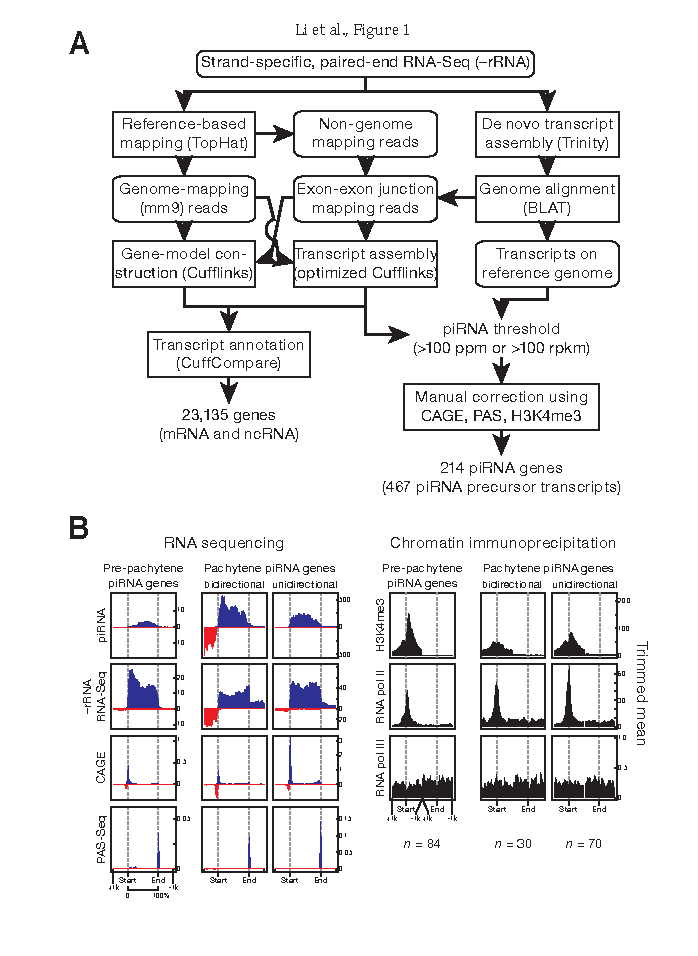
\includegraphics{Figures/MolCel/MolCel2013_Fig1.eps}
      \caption[piRNA Precursors are RNA Pol II Transcripts]
      {
        piRNA Precursors are RNA Pol II Transcripts\\[0.25cm]
        (A) Strategy to assemble the mouse testis transcriptome. Rectangles with rounded corners, input or output data; rectangles, processes. Decisions are shown without boxing.(B) Aggregated data for piRNA-producing transcripts (5\% trimmed mean). Oxidized small RNA (>23 nt) sequencing data were used to detect piRNAs; transcript abundance was measured using total RNA depleted of rRNA (RNA-seq). RNA Pol III data were from SRA001030. Dotted lines show the transcriptional start site (Start) and site of polyadenylation (End). See also Figure \ref{MolCel:fig:MolCelS1}.
        }
      \label{MolCel:fig:MolCelF1}
      \end{figure}
    \begin{figure} % Figure S1
      \centering 
      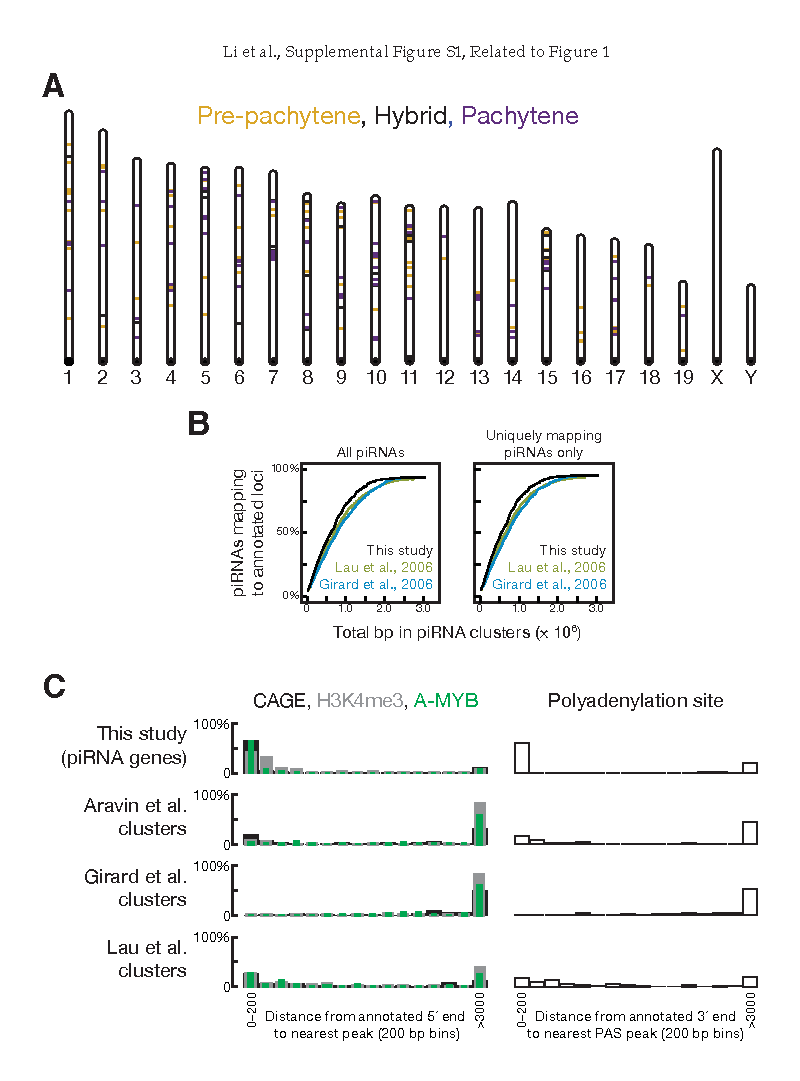
\includegraphics{Figures/MolCel/MolCel2013_FigS1.eps}
      \caption[The Major piRNA-Producing Genes of the Post-Partum Mouse Testis]
      {
        See subsection \ref{MolCel:subsubsec:cap:Figure S1} for full figure caption.
        }
      \label{MolCel:fig:MolCelS1}
      \end{figure}

    To identify the transcripts that produce piRNAs, we sequenced piRNAs from six developmental stages of mouse testes (10.5 dpp, 12.5 dpp, 14.5 dpp, 17.5 dpp, 20.5 dpp, and adult) and mapped them to the assembled transcripts. The first round of spermatogenesis proceeds synchronously among the tubules of the testis: mouse testes at 10.5 dpp advance no further than the zygotene stage (staging according to \citep{NEBEL1961}; 12.5 dpp to the early pachytene; 14.5 dpp to the middle pachytene; 17.5 to the late pachytene; and 20.5 dpp to the round spermatid stage. For each stage, we prepared two sequencing libraries: one comprising all small RNAs and one in which oxidation was used to enrich for piRNAs by virtue of their 2\textprime-O-methyl-modified 3\textprime~termini \citep{Ghildiyal2008}.

    To qualify as a piRNA-producing transcript, an assembled RNA was required to produce either a sufficiently high piRNA abundance (>100 ppm; parts per million uniquely mapped reads) or density (>100 rpkm; reads per kilobase of transcript per million uniquely mapped reads). These criteria retained both long transcripts producing an abundance of piRNAs and short transcripts generating many piRNAs per unit of length. To refine the termini of each piRNA-producing transcript, we supplemented the RNA-seq data with high-throughput sequencing of the 5\textprime~ends of RNAs bearing an N(5\textprime~)ppp(5\textprime~)N cap structure (cap analysis of gene expression; CAGE) and the 3\textprime~ends of transcripts preceding the poly(A) tail (polyadenylation site sequencing; PAS-seq). The assembled piRNA-producing transcripts likely correspond to continuous RNAs in vivo because the CAGE library used to annotate transcript 5\textprime~ends was constructed after two rounds of poly(A) selection. Thus, the RNA molecules in the library derive from complete transcripts extending from the 5\textprime~cap to the poly(A) tail (Figure \ref{MolCel:fig:MolCelF1}B). Conventional 5\textprime~and 3\textprime~RACE (rapid amplification of cDNA ends) analysis of piRNA-producing transcripts confirmed the ends of 16 loci (data not shown). To provide additional confirmation of the 5\textprime~end of each piRNA-producing transcript, we also determined the locations of histone H3 bearing trimethylated lysine 4 (H3K4me3), a histone modification associated with RNA Pol II transcription start sites \cite{Guenther2007}.

    \subsubsection{Caption for Figure \ref{MolCel:fig:MolCelS1}}
      \label{MolCel:subsubsec:cap:Figure S1}
      (A) Positions of the 214 major piRNA-producing genes on the 19 autosomes of mice. We detected no loci on the X or Y chromosomes. (B) Cumulative distributions for all piRNAs and for uniquely mapping piRNAs comparing the piRNA loci defined by our methods and by previous approaches \citep{Girard2006, Lau2006}. (C) Histogram of distances (in 200 bp bins) from the annotated 5\textprime~or 3\textprime~end of a piRNA gene (this study) or cluster to the nearest peak of reads from high-throughput sequencing for transcript 5\textprime~(CAGE-seq) or 3\textprime~(PAS-seq) ends, transcription start sites (H3K4me3) or A-MYB binding.

  \subsection{piRNA Precursor RNAs are Canonical RNA Pol II Transcripts}
    \label{MolCel:subsec:Precursors are Pol II Txs}

    The presence of 5\textprime~caps and poly(A) tails and the binding of histone H3K4me3 to the genomic DNA immediately upstream of the transcription start site of each piRNA locus suggest that piRNA transcripts are produced by RNA pol II \ref{MolCel:fig:MolCelF1}. Moreover, using antibodies to RNA pol II but not RNA pol III, ChIP-seq showed a peak at the transcription start site as well as polymerase occupancy across the entire piRNA gene (Figure \ref{MolCel:fig:MolCelF1}B; \citep{Kutter2011}. We conclude that piRNA transcripts are conventional RNA pol II transcripts bearing 5\textprime~caps and 3\textprime~poly(A) tails.

  \subsection{A Transcript-based Set of piRNA Loci}
    \label{MolCel:subsec:A TX-based set of piRNA loci}

    Our transcriptome assembly yielded 467 piRNA-producing transcripts that define 214 genomic loci (Figure \ref{MolCel:fig:MolCelS1}A and Table S1). Among the \textasciitilde2.2 million distinct piRNA species and \textasciitilde8.8 million piRNA reads from the adult mouse testis, the 214 genomic loci account for 95\% of all piRNAs.

    Previous studies defined piRNA clusters based solely on small RNA sequencing data \citep{Girard2006, Lau2006, Aravin2007a}. Our approach differs in that it (1) uses RNA-seq data, whose greater read length facilitates the identification of introns, allowing us to define the architecture of piRNA precursor transcripts and (2) uses CAGE, PAS-seq, and H3K4me3 ChIP-seq data to refine the 5\textprime~and 3\textprime~ends of the piRNA transcripts. Consequently, the piRNA loci presented here account for more piRNAs using fewer genomic base pairs than those previously defined (Figures \ref{MolCel:fig:MolCelS1}B and \ref{MolCel:fig:MolCelS1}C; \citep{Lau2006, Girard2006}. Our piRNA-producing loci include 41 piRNA loci that escaped previous detection \citep{Girard2006, Lau2006, Aravin2007a}, 37 of which contain introns. The 41 loci account for 2\% of piRNAs at 10.5 dpp and 0.36\% in the adult testis.

  \subsection{Three Classes of piRNAs During Post-Natal Spermatogenesis}
    \label{MolCel:subsec:Three Classes of piRNAs in testes}

    Mice produce three PIWI proteins: MIWI2 (PIWIL4), which binds piRNAs in perinatal testis \citep{Carmell2007, Aravin2008a}; MILI (PIWIL2), which binds piRNAs at least until the round spermatid stage of spermatogenesis \citep{Kuramochi-Miyagawa2004, Aravin2006, Aravin2007a}; and MIWI (PIWILl), which is first produced during the pachytene stage of meiosis \citep{Deng2002c}. From 10.5 to 20.5 dpp, piRNA abundance increases and longer piRNAs appear, reflecting a switch from MILI-bound piRNAs, which have a 26-27 nt modal length \citep{Montgomery1998, Aravin2006, Aravin2008a, Robine2009}, to MIWI-bound piRNAs, which have a 30 nt modal length (Figure \ref{MolCel:fig:MolCelS2}A; \citep{Reuter2009, Robine2009}. This switch occurs at the pachytene phase of meiosis. MILI-bound pre-pachytene piRNAs predominate before the onset of pachynema; at the pachytene and round spermatid stages, most piRNAs are MIWI-bound pachytene piRNAs.

    We used hierarchical clustering to analyze the change in piRNA abundance from 10.5 to 20.5 dpp for the 214 genes defined by our data (Figures \ref{MolCel:fig:MolCelF2}A and \ref{MolCel:fig:MolCelS2}A and Table S2). Three types of piRNA-producing genes were identified according to when their piRNAs first accumulate and how their expression changes during spermatogenesis: 84 pre-pachytene, 100 pachytene, and 30 hybrid loci. At 10.5 dpp, the earliest time we evaluated, 84 genes dominate piRNA production (median piRNA abundance per gene = 16 rpkm; Figure \ref{MolCel:fig:MolCelF2}B). Nearly all (81 out of 84) were congruent with protein-coding genes. The 84 pre-pachytene piRNA genes account for 13\% of piRNAs at 10.5 dpp, but only 0.31\% of piRNAs in the adult testis. Of the pre-pachytene piRNAs accounted for by the 84 loci, 15\% derive from 31 piRNA-producing genes that, to our knowledge, have not previously been described.

    \begin{figure} % Figure 2
      \centering 
      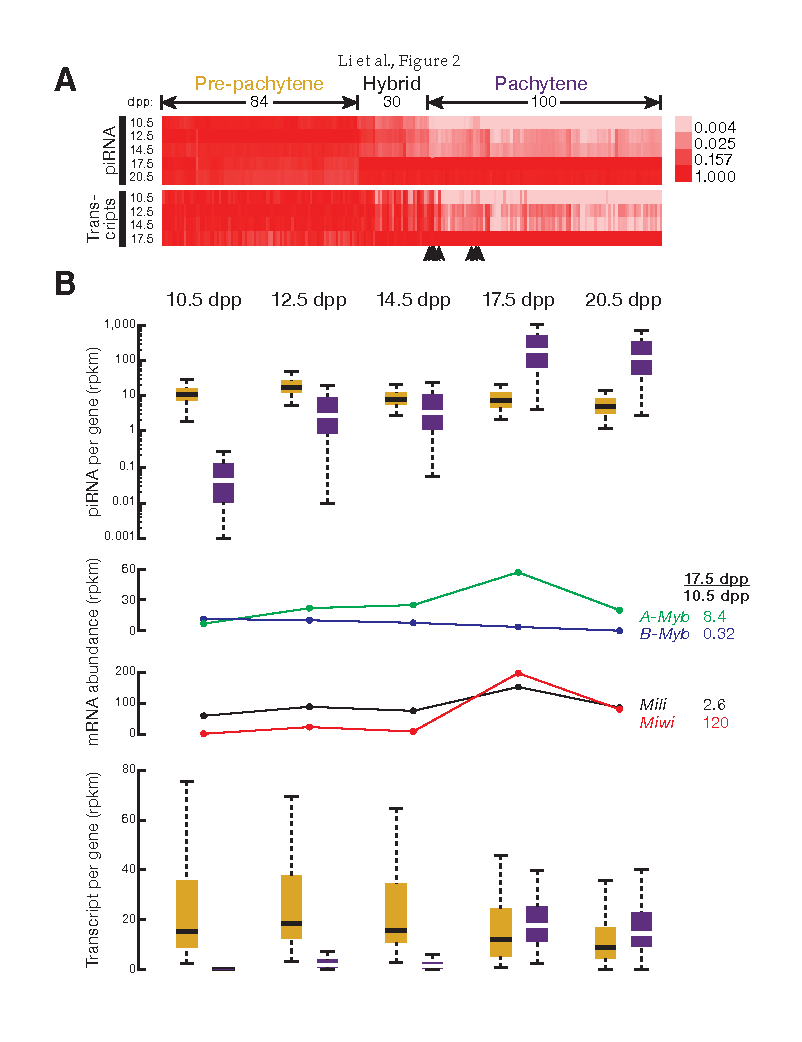
\includegraphics{Figures/MolCel/MolCel2013_Fig2.eps}
      \caption[Three Classes of piRNA-Generating Loci]
      {
        See subsection \ref{MolCel:subsubsection:cap:Figure F2} for full figure caption.
        }
      \label{MolCel:fig:MolCelF2}
      \end{figure}
    \begin{figure}\tiny % Figure S2
      \centering 
      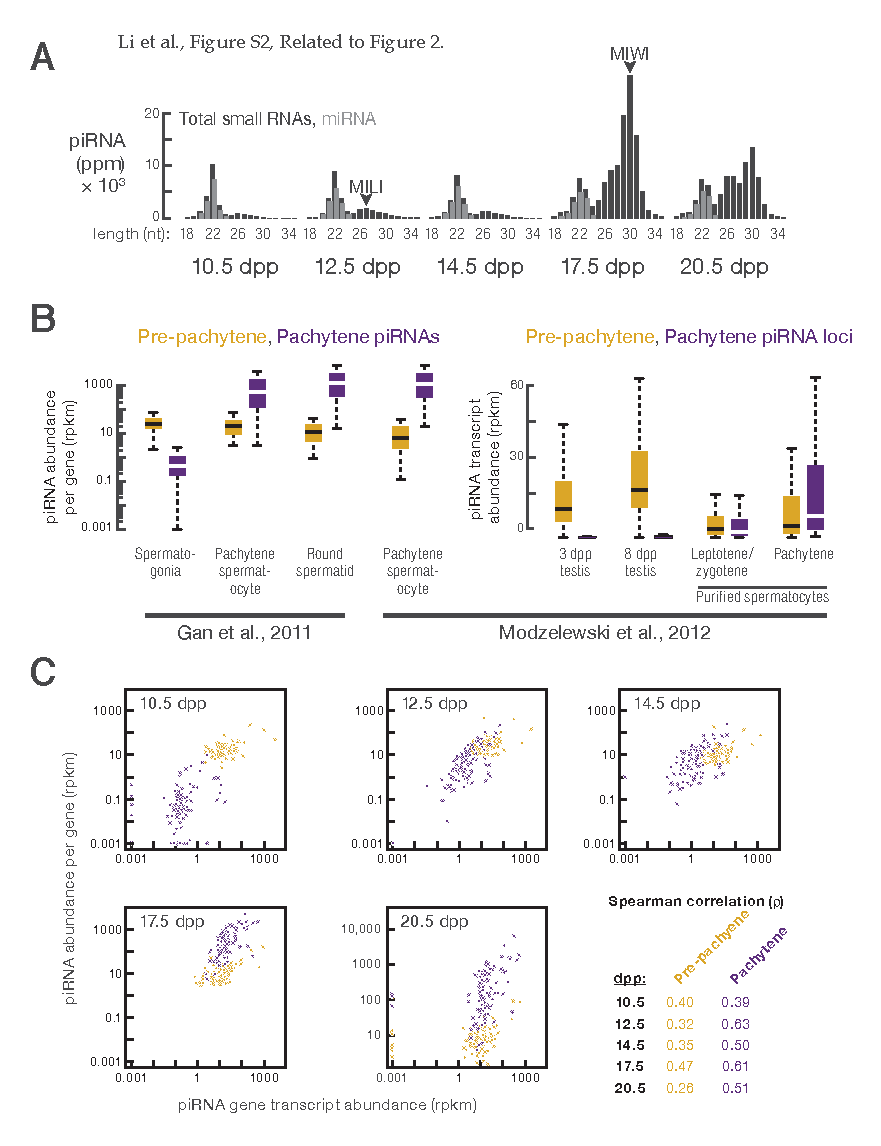
\includegraphics{Figures/MolCel/MolCel2013_FigS2.eps}
      \caption[Pre-pachytene piRNAs Persist in Pachytene Spermatocytes]
      {
        See subsection \ref{MolCel:subsubsection:cap:Figure S2} for full figure caption.
     	  }
      \label{MolCel:fig:MolCelS2}
      \end{figure}

    A parallel analysis of piRNA precursor transcription using RNA-seq (>100 nt) corroborated the classification based on piRNA abundance; of the 100 piRNA genes classified as pachytene based on the developmental expression profile of their piRNAs, 93 were grouped as pachytene according to the developmental expression profile of their transcripts. Of these 93, 89 are intergenic. All 84 piRNA genes designated pre-pachytene using piRNA data were classified as pre-pachytene according to their transcript abundance.

    Despite their name, pre-pachytene piRNAs were readily detected in >90\% and \textasciitilde95\% pure pachytene spermatocytes, as well as round spermatids (Figure \ref{MolCel:fig:MolCelS2}B; \citep{Gan2011,Modzelewski2012}. Transcript abundance from the 84 pre-pachytene loci was high at 3 dpp (median abundance = 11 rpkm), higher by 8 dpp (18 rpkm), and lower in purified leptotene/zygotene spermatocytes (3.3 rpkm; \ref{MolCel:fig:MolCelS2}B). Yet piRNA precursor transcripts were readily detectable in purified pachytene spermatocytes at a level (4.6 rpkm) comparable to that in purified leptotene/zygotene spermatocytes (Figure \ref{MolCel:fig:MolCelS2}B);  \citep{Gan2011,Modzelewski2012}. From 10.5 to 20.5 dpp, the steady-state level of pre-pachytene piRNA precursor transcripts remained constant (Figure \ref{MolCel:fig:MolCelS2}B).

    Finally, the abundance of pre-pachytene piRNA precursor transcripts was better correlated with pre-pachytene piRNA abundance at 17.5 dpp ($\rho$ = 0.47), when pachytene spermatocytes compose a larger fraction of the testis, than at 10.5, 12.5, or 14.5 dpp (0.32 $\ge \rho \le$ 0.40; Figure \ref{MolCel:fig:MolCelS2}C). Our data suggest that the pre-pachytene loci continue to be transcribed and processed into piRNAs long after spermatocytes enter the pachytene stage of meiosis. Thus, the name pre-pachytene piRNA is a misnomer that should be retained only for historical reasons.

    Hierarchical clustering identified 100 pachytene genes whose piRNAs emerge at 12.5 dpp, 2 days earlier than previously reported \citep{Girard2006}. Nearly all the pachytene genes are intergenic (93 out of 100). piRNA expression from pachytene piRNA genes peaks at 17.5 dpp (Figure \ref{MolCel:fig:MolCelF2}B). Overall, the median abundance of piRNAs from these 100 loci increased >6,000-fold from 10.5 to 17.5 dpp. Transcripts from pachytene genes were low at 10.5 dpp (median abundance = 0.15 rpkm) and increased 116-fold from 10.5 to 17.5 dpp. From 10.5 to 20.5 dpp, the dynamics of pachytene piRNA abundance from each piRNA gene correlated with the increase in abundance of its precursor transcripts (0.39 $\ge \rho \le$  0.63; $\rho value \le 7.3 x 10-5$; Figure \ref{MolCel:fig:MolCelS2}C). The 100 pachytene genes account for 92\% of piRNAs in the adult testis, making it unlikely that biologically functional pachytene piRNAs originate from thousands of genomic loci \citep{Gan2011}. Figures \ref{MolCel:fig:MolCelF3} and \ref{MolCel:fig:MolCelS3} provide examples of pachytene and pre-pachytene piRNA genes defined by our data.

    \begin{landscape}
    \begin{figure} % Figure 3
      \centering 
      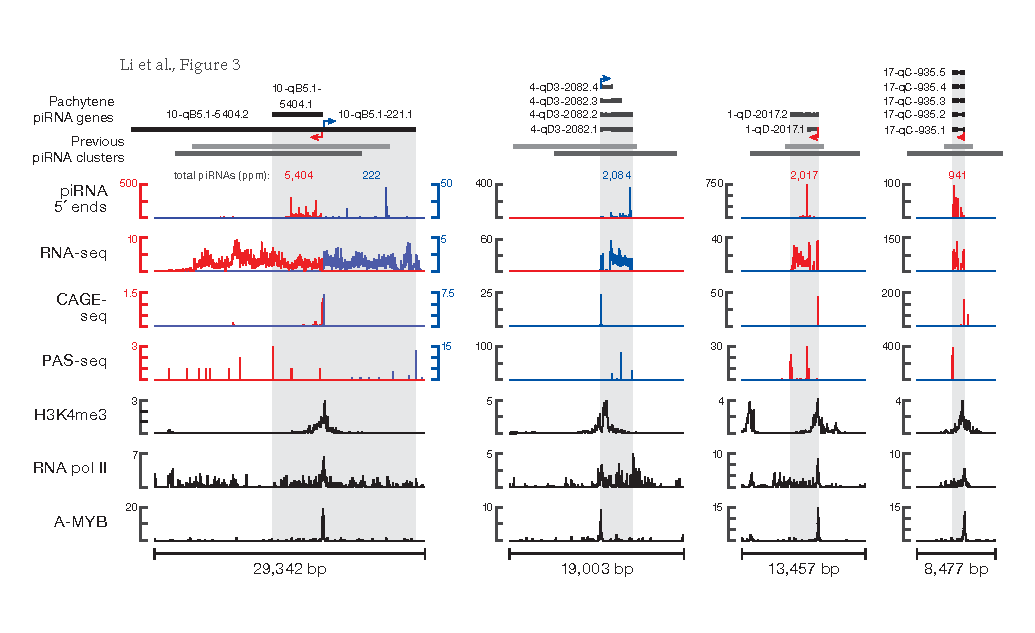
\includegraphics{Figures/MolCel/MolCel2013_Fig3.eps}
      \caption[Examples of Pachytene piRNA Genes]
      {
	      Previous cluster boundaries are from \citet{Lau2006} in gray and \citet{Girard2006} in  dark gray).
      	}
     	\label{MolCel:fig:MolCelF3}
   		\end{figure}

    \begin{figure} % Figure S3
      \centering 
      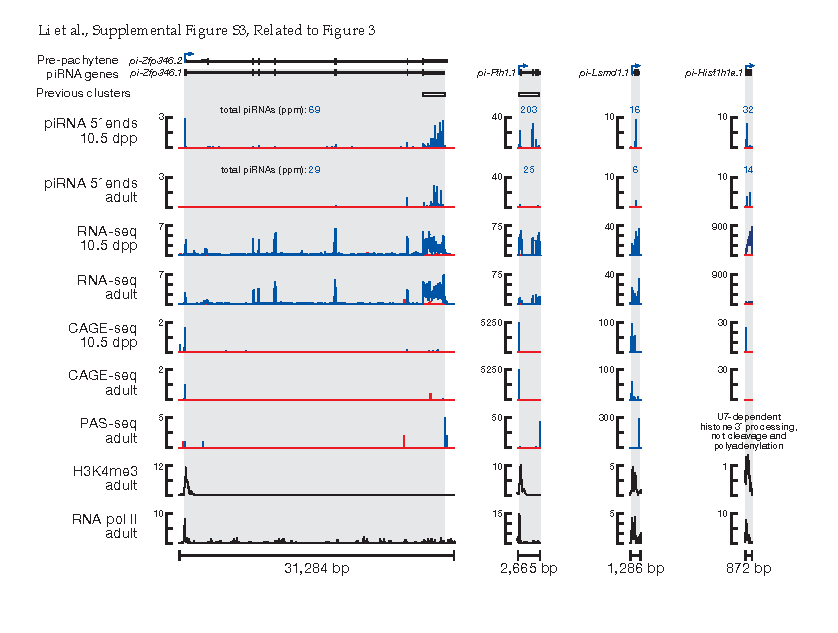
\includegraphics{Figures/MolCel/MolCel2013_FigS3.eps}
      \caption[Examples of Pre-Pachytene piRNA Genes]
      {
      	Previous cluster boundaries are from \citet{Lau2006} in gray and \citet{Girard2006} in  dark gray).
      	}
      \label{MolCel:fig:MolCelS3}
    	\end{figure}
    \end{landscape}

    Hierarchical clustering detected a third class, hybrid piRNAs, which derives from 30 genes with characteristics of both pre-pachytene and pachytene piRNA loci. Like pre-pachytene, hybrid piRNAs were detected at 10.5 dpp (median abundance = 3.7 rpkm) and in purified spermatogonia \citep{Gan2011}. Like pachytene piRNAs, hybrid piRNA abundance increased during the pachytene stage of meiosis, but the increase was delayed until late (17.5 dpp) rather than early pachynema (14.5 dpp). Overall, piRNAs from hybrid genes increased >10-fold from 14.5 to 17.5 dpp. The median abundance of piRNAs from hybrid piRNA genes ranged from 90-120 rpkm in purified pachytene spermatocytes, >20-fold greater than their median abundance in spermatogonia \citep{Gan2011,Modzelewski2012}. Moreover, hybrid piRNA precursor transcripts were readily detected in purified pachytene spermatocytes (median abundance = 9.0 rpkm; \citep{Modzelewski2012}).

    \subsubsection{Caption for Figure \ref{MolCel:fig:MolCelF2}}
      \label{MolCel:subsubsection:cap:Figure F2}
      (A) Normalized piRNA density (rpkm) for each piRNA-producing gene is shown as a heatmap across the developmental stages. Hierarchical clustering divided the genes into three classes. Arrowheads mark seven pachytene piRNA genes that were not classified as pachytene according to the change in the abundance of their precursor RNAs from 10.5 to 17.5 dpp.(B) Top: box plots present piRNA density per gene as spermatogenesis progresses (here and elsewhere, pre-pachytene in yellow and pachytene in purple). Middle: expression of \amyb{}, \bmyb{}, \mili{}, and \miwi{} was measured by RNA-seq. Bottom: box plots present piRNA precursor expression per gene, measured by RNA-seq, from 10.5 to 20.5 dpp. See also Figure \ref{MolCel:fig:MolCelS2} and Table S2.

    \subsubsection{Caption for Figure \ref{MolCel:fig:MolCelS2}}
      \label{MolCel:subsubsection:cap:Figure S2}
      (A) As shown previously by others using lower temporal resolution, the modal length of piRNAs increases as spermatogenesis proceeds to more advanced stages. (B) Total piRNA rpkm abundance and piRNA transcript abundance per locus by class, from purified spermatogonia, spermatocytes, round spermatids, and 3 dpp and 8 dpp testis \citep{Gan2011, Modzelewski2012}. (C) Correlation between piRNA abundance per locus and piRNA precursor transcription from 10.5 to 20.5 dpp. Throughout the Figures, gold indicates pre-pachytene and purple indicates pachytene piRNA loci.

  \subsection{\amyb{} Regulates Pachytene piRNA Precursor Transcription}
    \label{MolCel:subsec:A-Myb controls Pachytene precursor Tx}

    The coordinated increase in pachytene piRNA precursor transcripts suggests their regulation by a common transcription factor or factors. Among the 100 pachytene piRNA genes, 15 pairs (30 genes) are divergently transcribed. The 5\textprime~ends of the piRNA precursor RNAs from each pair are close in genomic distance (median = 127 bp), suggesting that a shared promoter lies between the two transcription start sites.
     
    We took advantage of the unique genomic organization of these 15 pairs of divergently transcribed piRNA genes to search for sequence motifs common to their promoters. The MEME algorithm \citep{Bailey1994} revealed a motif highly enriched in these bidirectional promoters (E = 8.3 x 10$^{12}$; Figure \ref{MolCel:fig:MolCelF4}A). This motif matches the binding site of the Myb family of transcription factors (Figure \ref{MolCel:fig:MolCelF4}A; \citep{Gupta2007, Newburger2009}. The Myb motif is not restricted to bidirectional promoters; MEME identified the same motif using the promoters of all pachytene piRNA genes (E = 9.1 x 10$^{-28}$; Figure \ref{MolCel:fig:MolCelF4}B).

    \begin{figure} % Figure 4
      \centering 
      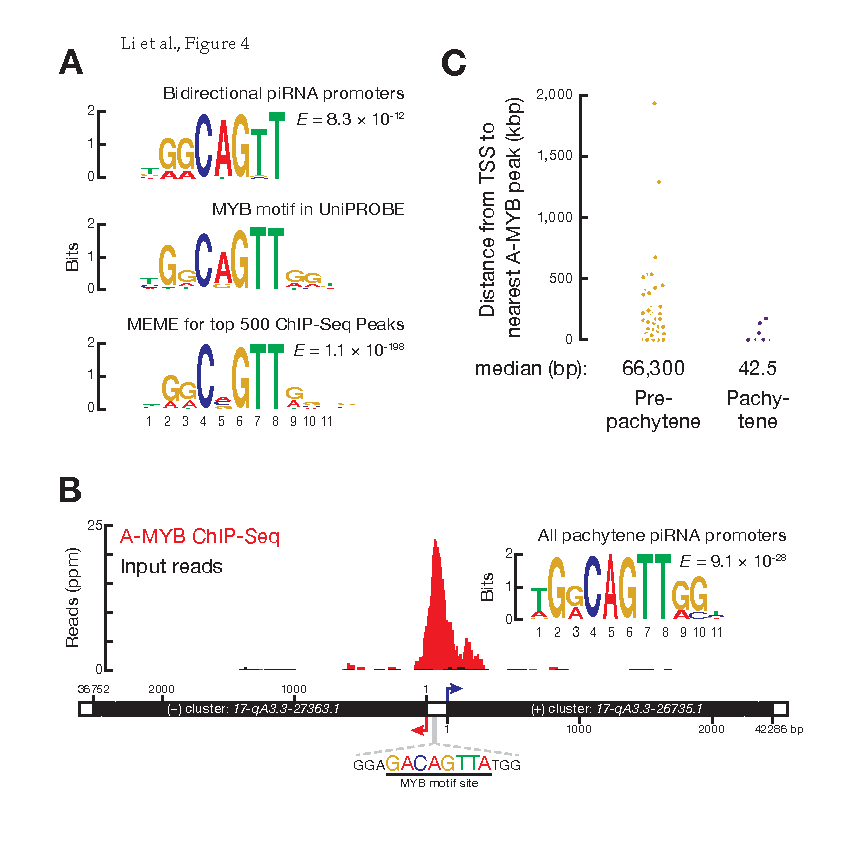
\includegraphics{Figures/MolCel/MolCel2013_Fig4.eps}
      \caption[A-MYB Binds the Promoters of Pachytene piRNA Genes]
      {
       (A) Top: MEME identified a sequence motif in the bidirectional promoters of the 15 pairs of divergently transcribed pachytene piRNA genes. E value computed by MEME measures the statistical significance of the motif. Middle: Myb motif from the mouse UniPROBE database. Bottom: MEME-reported motif for the top 500 (by peak score) A-MYB ChIP-seq peaks from adult mouse testes.(B) A-MYB ChIP-seq data for the common promoter of the divergently transcribed pachytene piRNA genes \textit{17-qA3.3-27363.1} and \textit{17-qA3.3-26735.1}.(C) The distance from the annotated transcription start site (TSS) of each piRNA gene to the nearest A-MYB peak. See also Figure \ref{MolCel:fig:MolCelS4}.
      	}
      \label{MolCel:fig:MolCelF4}
    	\end{figure}
    \begin{figure} % Figure S4
      \centering 
      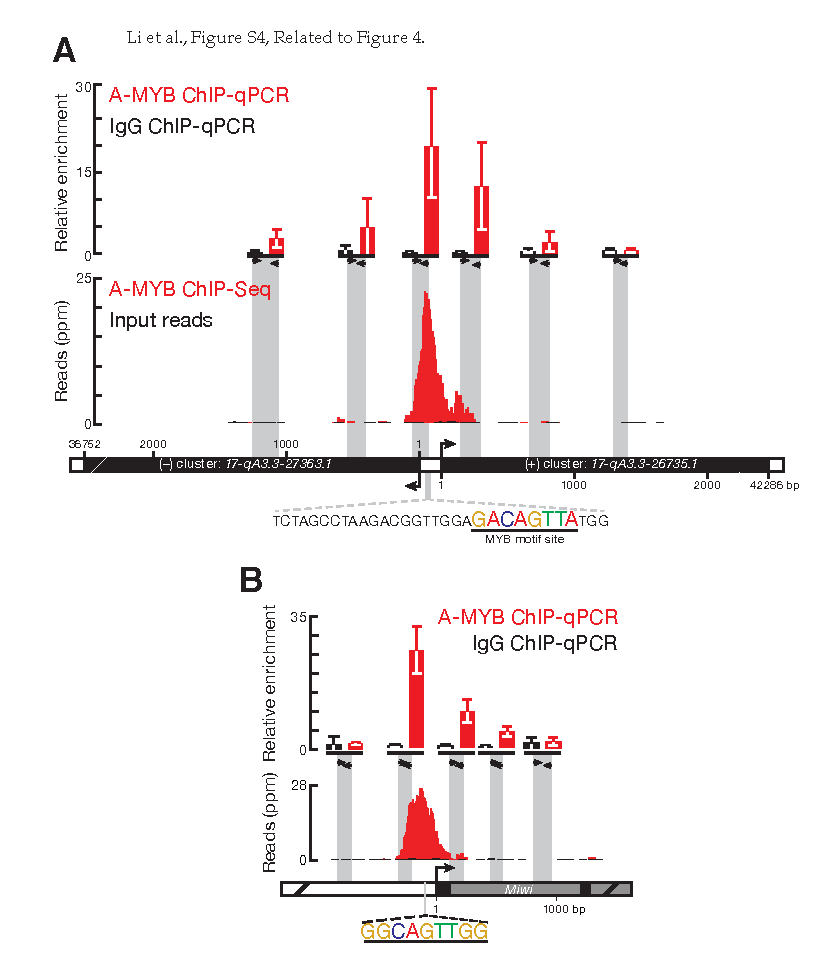
\includegraphics{Figures/MolCel/MolCel2013_FigS4.eps}
      \caption[ChIP-qPCR Confirms ChIP-seq Data]
      {
     	 (A) A-MYB binds to the common promoter of divergently transcribed pachytene piRNA loci \textit{17-qA3.3-27363.1} and \textit{17-qA3.3-26735.1}. The abundance of DNA fragments at the amplified region relative to a control region (mean $\pm$ standard deviation; n = 3) was measured by qPCR (top). The A-MYB ChIP-seq (red) and input (black) data for this pair of genes is presented as in Figure \ref{MolCel:fig:MolCelF4}B. (B) ChIP-seq and qPCR were as in (A), but for the promoter region of \miwi{} (Piwil1). Also shown is the RefSeq gene model. Exons, black; introns, gray.
     	 }
      \label{MolCel:fig:MolCelS4}
    	\end{figure}

    The Myb transcription factor family is conserved among eukaryotes. Like other vertebrates, mice produce three Myb proteins, A-MYB (MYBL1), B-MYB (MYBL2), and C-MYB (MYB), each with a distinct tissue distribution \citep{Mettus1994, Trauth1994, Latham1996, Oh1999}. Testes produce both A- and B-MYB proteins. Multiple lines of evidence implicate A-MYB, rather than B-MYB, as a candidate for regulating pachytene piRNA transcription. First, the expression of \amyb{} during spermatogenesis resembles that of pachytene piRNAs: \amyb{} transcripts appear at \textasciitilde12.5 dpp and peak at 17.5 dpp (Figure \ref{MolCel:fig:MolCelF2}B; \citep{Bolcun-Filas2011}. The expression of \amyb{} messenger RNA (mRNA) increases \textasciitilde15-fold from 8 dpp to 19 dpp, whereas \bmyb{} mRNA expression remains constant and low during the same time frame and into adulthood \citep{Horvath2009}. Our RNA-seq data (Figure \ref{MolCel:fig:MolCelF2}B) corroborate these findings. Indeed, in our RNA-seq analysis of adult testes, \amyb{} mRNA was 24-fold more abundant than \bmyb{}. Second, a testis-specific \amyb{} point-mutant allele, \mybrepro, which is caused by a cytosine-to-adenine transversion that changes alanine 213 to glutamic acid, leads to meiotic arrest at the pachytene stage with subtle defects in autosome synapsis; \amyb{} null mutant mice have defects in multiple tissues, including the testis and the mammary gland \citep{Toscani1997, Bolcun-Filas2011}. Third, our RNA-seq analysis of \amyb{} mutant testes shows that there is no significant change in \bmyb{} expression in the mutant, compared to the heterozygous controls, at 14.5 or 17.5 dpp. Finally, B-MYB protein is not detectable in pachytene spermatocytes \citep{Horvath2009}.

    To assess more directly the role of A-MYB in pachytene piRNA precursor transcription, we used anti-A-MYB antibody to perform ChIP followed by high-throughput sequencing of the A-MYB-bound DNA. The anti-A-MYB antibody is specific for A-MYB, and the peptide used to raise the antibody is not present in B-MYB. The model-based analysis of ChIP-seq (MACS) algorithm \citep{Zhang2008} reported 3,815 genomic regions with significant A-MYB binding (false discovery rate, FDR < 10$^{25}$); we call these regions A-MYB peaks or peaks. Among the 500 peaks with the lowest FDR values, 394 (80\%) contained at least one significant site ($\rho < 10^{4}$) for the MYB binding motif (Figure \ref{MolCel:fig:MolCelF4}A). Figure \ref{MolCel:fig:MolCelF4}B shows an example of such an A-MYB peak at the bidirectional promoter of the divergently transcribed pair of pachytene piRNA genes \textit{17-qA3.3-27363.1} and \textit{17-qA3.3-26735.1}. A-MYB occupancy of this genomic site was confirmed by ChIP and quantitative PCR (ChIP-qPCR) (Figure \ref{MolCel:fig:MolCelS4}A).

    The median distance from the transcription start site to the nearest A-MYB peak was \textasciitilde43 bp for the 100 pachytene piRNA genes but >66,000 bp for the 84 pre-pachytene genes (Figure \ref{MolCel:fig:MolCelF4}C). Our data suggest that during mouse spermatogenesis A-MYB binds to the promoters of both divergently and unidirectionally transcribed pachytene piRNA genes.

    To test the idea that A-MYB promotes transcription of pachytene, but not pre-pachytene, piRNA genes, we used RNA-seq to measure the abundance of RNA > 100 nt long from the testes of \amyb{} point-mutant (\mybrepro) mice and their heterozygous littermates (Figure \ref{MolCel:fig:MolCelF5}). Pachytene piRNA precursor transcripts—both divergently and unidirectionally transcribed—were significantly depleted in \amyb{} mutant testes compared to the heterozygotes: the median decrease was 45-fold at 14.5 dpp (q = 1.1 x 10$^{-13}$) and 248-fold at 17.5 dpp (q = 3.9 x 10$^{-23}$). The abundance of pre-pachytene piRNA transcripts was not significantly changed (q $\ge $ 0.34). The binding of A-MYB to the promoters of pachytene piRNA genes, together with the depletion of pachytene piRNA transcripts in the \amyb{} mutant, further supports the view that A-MYB directly regulates transcription of pachytene piRNA genes.

  \subsection{\amyb{} Regulates Pachytene piRNA Production}
    \label{MolCel:subsec:A-Myb regulates pachytene piRNA production}

    To test the consequences of the loss of piRNA precursor transcripts, we measured piRNA abundance in the \amyb{} mutant. Like pachytene piRNA precursor transcription, pachytene piRNA abundance significantly decreased in mutant testes. At 14.5 dpp, median piRNA abundance per pachytene gene decreased 87-fold in \amyb{} homozygous mutant testes compared to heterozygotes ($\rho < 2.2 X 10^{-16}$; Figure \ref{MolCel:fig:MolCelF5}. By 17.5 dpp, median pachytene piRNA abundance was >9,000 times lower in the \amyb{} mutant than the heterozygotes (P < 2.2 x 10$^{-16}$). In contrast, pre-pachytene piRNA levels were essentially unaltered. Figure 6 presents examples of the effect at 14.5 and 17.5 dpp of the \amyb{} mutant on piRNA precursor transcript and mature piRNA abundance for one pre-pachytene and three pachytene piRNA genes.

    \begin{figure} % Figure 5
      \centering 
      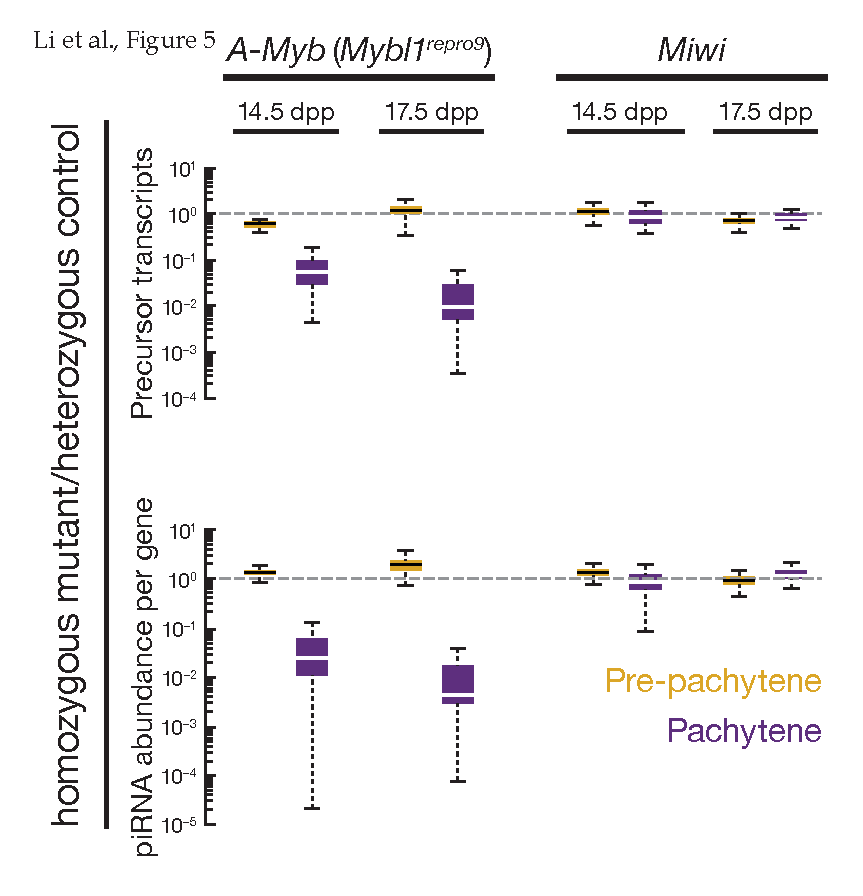
\includegraphics{Figures/MolCel/MolCel2013_Fig5.eps}
      \caption[Pachytene piRNAs and Precursors Decrease in \amyb{} Mutant Testes]
      {
     	 The change in transcript or piRNA abundance per gene in \amyb{} (n = 3) and \miwi{} (n = 1) mutants compared to heterozygotes in testes isolated at 14.5 and 17.5 dpp. See also Figure \ref{MolCel:fig:MolCelS5}.
     	 }
      \label{MolCel:fig:MolCelF5}
   	  \end{figure}
    \begin{figure} % Figure S5
      \centering 
      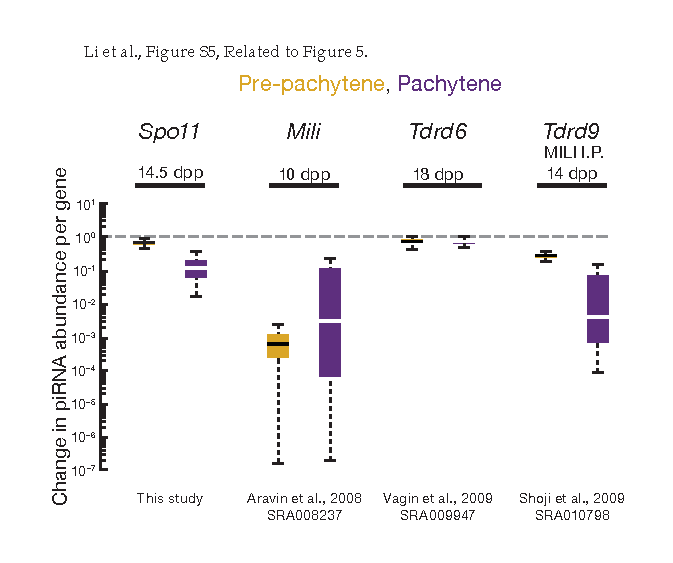
\includegraphics{Figures/MolCel/MolCel2013_FigS5.eps}
      \caption[Change in piRNA Expression in \spo{}, \miwi{}, \textit{Tdrd6}, and \textit{Tdrd9} Mutants]
      {
      Change in piRNA abundance per locus (rpkm) for \spo{} (14.5 dpp), \miwi{} (\textit{Piwil2}; 10.5 dpp), \textit{Tdrd6} (18 dpp), and \textit{Tdrd9} (14 dpp) mutants compared to heterozygous controls.
      }
      \label{MolCel:fig:MolCelS5}
 	   \end{figure}

    Our data show that A-MYB binds to the promoters of pachytene piRNA genes; \amyb{}, \miwi{}, and pachytene piRNA precursor transcription begins at 12.5 dpp; and \amyb{} mutant spermatocytes reach pachynema with subtle defects in autosome synapsis \citep{Bolcun-Filas2011}. Could pachytene piRNA depletion nonetheless be an indirect consequence of the meiotic arrest caused by the \amyb{} mutant? To test this possibility, we sequenced small RNAs from \spo{} mutant testes, which failed to generate double-stranded DNA breaks at the leptotene stage and display a meiotic arrest \citep{Baudat2000c,Romanienko2000}. The median abundance of piRNAs from pre-pachytene genes did not decrease at 14.5 dpp. By 17.5 dpp, piRNA from pachytene genes decreased just 5.9-fold in the \spo{} mutant testes compared to the heterozygotes (Figure \ref{MolCel:fig:MolCelS5}). We note that A-MYB protein abundance is reduced in the \spo{} mutant \citep{Bolcun-Filas2011}.

    \textit{Trip13} is required to complete the repair of double-strand DNA breaks on fully synapsed chromosomes. \textit{Trip13} mutants display a meiotic arrest similar to that in \amyb{} mutant testes \citep{Li2007}: pachytene arrest with synapsed chromosomes. To further test whether the loss of pachytene piRNA precursor transcripts in \amyb{} mutants reflects a general effect of meiotic arrest, we measured piRNA precursor transcript abundance in \textit{Trip13} mutant testes at 17.5 dpp. Unlike \amyb{}, piRNA precursor transcripts were readily detectable in the \textit{Trip13} mutant (Figure \ref{MolCel:fig:MolCelS6}). We conclude that the loss of pachytene piRNA precursor transcripts and piRNAs in \amyb{} mutant testes is a direct consequence of the requirement for A-MYB to transcribe pachytene piRNA genes and not a general feature of meiotic arrest at the pachytene stage.

  \subsection{\amyb{} Regulates Expression of piRNA Biogenesis Factors}
    \label{MolCel:subsec:A-Myb regulations piRNA machinery}

    The \amyb{} mutant more strongly affected pachytene piRNA accumulation than it did the steady-state abundance of the corresponding piRNA precursor transcripts (Figure \ref{MolCel:fig:MolCelF5}; the median decrease in pachytene piRNA abundance was 2-fold greater at 14.5 dpp and 38-fold greater at 17.5 dpp than the decrease in the steady-state abundance of pachytene precursor transcripts (Table S1). These data suggest that A-MYB exerts a layer of control on piRNA accumulation beyond its role in promoting pachytene piRNA precursor transcription.

    \miwi{} has previously been proposed to be a direct target of A-MYB; \miwi{} mRNA abundance is reduced in A-MYB mutant testes, and ChIP microarray data place A-MYB on the \miwi{} promoter \citep{Bolcun-Filas2011}. Our RNA-seq data confirm that accumulation of \miwi{} mRNA requires A-MYB: \miwi{} mRNA decreased more than 50-fold in testes isolated from \amyb{} mutant mice at 14.5 dpp compared to their heterozygous littermates (Figures \ref{MolCel:fig:MolCelF7}A and \ref{MolCel:fig:MolCelS7} and Table S3). Furthermore, our ChIP data confirm that A-MYB binds the \miwi{} promoter in vivo (Figures \ref{MolCel:fig:MolCelF7}B, \ref{MolCel:fig:MolCelS4}B, and \ref{MolCel:fig:MolCelS7}). Like pachytene piRNAs, \miwi{} transcripts first appear at 12.5 dpp (Figure \ref{MolCel:fig:MolCelF2}B), and MIWI protein is first detected in testes at 14.5 dpp \citep{Deng2002c}. Loss of MIWI arrests spermatogenesis at the round spermatid stage \citep{Deng2002c}.

    A previous study reported that piRNAs fail to accumulate to wild-type levels in \miwi{} mutant testes \citep{Grivna2006}. However, our data suggest that the overall change in piRNA abundance caused by loss of MIWI is quite small: RNA-seq detected no change at 14.5 dpp (change in total piRNA abundance = 1.1; n = 2) and only a modest decrease at 17.5 dpp (change in total piRNA abundance = 0.58; n = 1). piRNAs from pachytene loci decreased just 2.7-fold at 14.5 dpp (p = 0.0046) and 3.5-fold at 17.5 dpp (p = 1.8 x 10-6) in \miwi{} mutant testes (Figure \ref{MolCel:fig:MolCelF5}). By comparison, pachytene piRNAs declined 87-fold at 14.5 dpp and 9,400-fold at 17.5 dpp in the \amyb{} mutant.

    Does the loss of MIWI affect piRNA precursor transcription? We measured transcript abundance and piRNA expression in \miwi{} null mutant testes at 14.5 and 17.5 dpp. In \miwi{}$^{-/-}$ testes, pachytene piRNA precursor transcripts were present at levels indistinguishable from \miwi{} heterozygotes (median change = 1.0- to 1.4-fold; q = 1; Figure \ref{MolCel:fig:MolCelF5}). Thus, loss of MIWI does not explain loss of pachytene piRNA precursor transcripts in \amyb{} mutant testes.

    \begin{figure} % Figure 6
      \centering 
      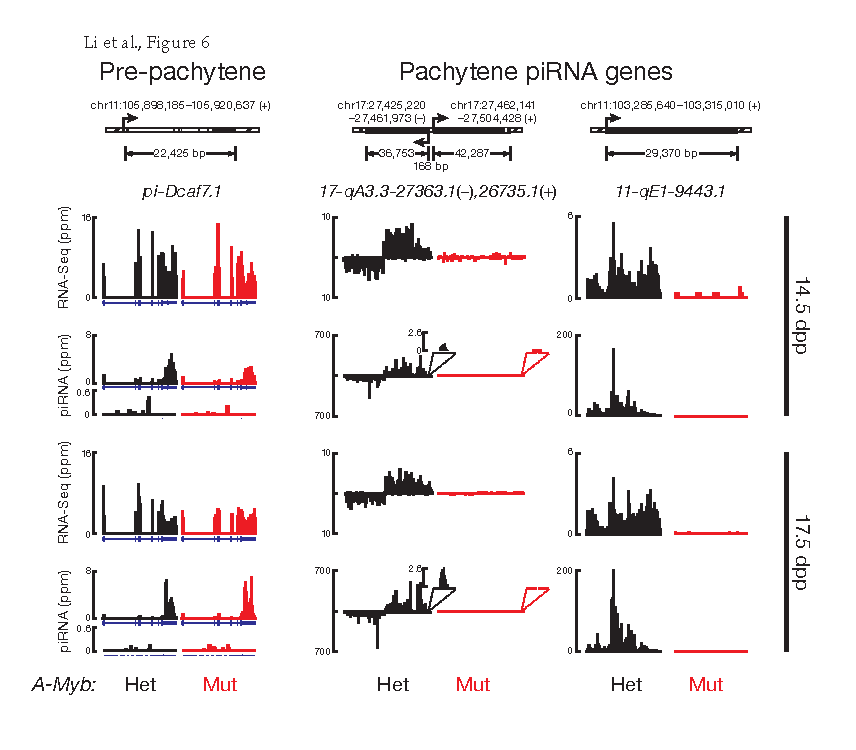
\includegraphics{Figures/MolCel/MolCel2013_Fig6.eps}
      \caption[Examples of the Effect of the \amyb{} Mutation on piRNA Expression]
      {
     	 Transcript and piRNA abundance in heterozygous (Het) and homozygous \amyb{} (Mut) point-mutant testes is shown for four illustrative examples at 14.5 and 17.5 dpp. Also shown is the abundance of piRNA sequencing reads that map to the exon-exon junctions. Gene \textit{11-qE1-9443} does not have an intron. Exons, blue boxes; splice junctions, gaps; the last exon is compressed and not to scale. See also Figure \ref{MolCel:fig:MolCelS6}.
     	 }
      \label{MolCel:fig:MolCelF6}
    	\end{figure}
    \begin{figure} % Figure S6
      \centering 
      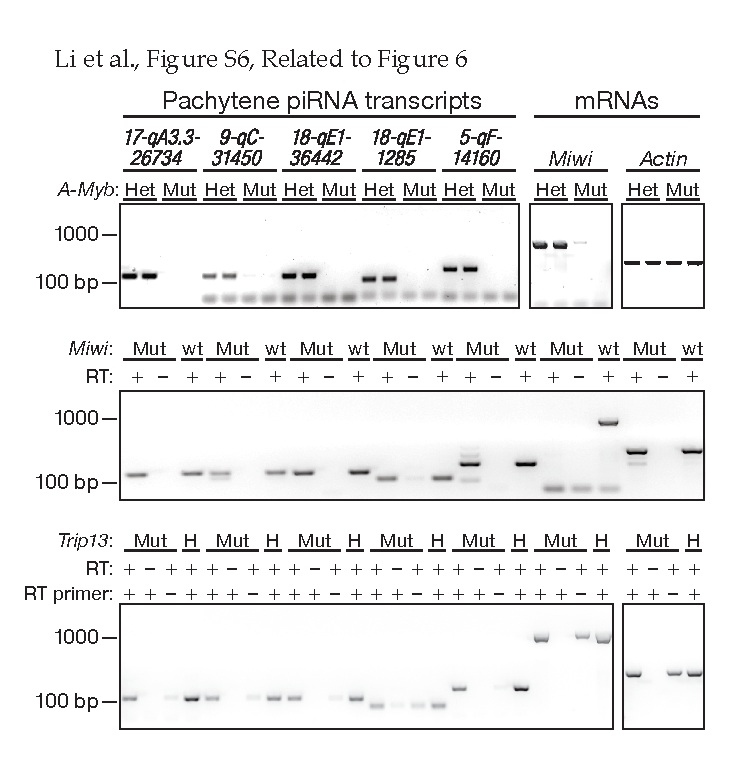
\includegraphics{Figures/MolCel/MolCel2013_FigS6.eps}
      \caption[Pachytene piRNA Precursor Abundance in \amyb{}, \miwi{}, and \textit{Trip13} Mutants]
      {
      Transcripts were detected in total RNA from adult testes by RT-PCR (using random primers) for five pachytene piRNA loci as well as \miwi{} and \textit{Actin}. Mut, mutant; Het or H, heterozygote; wt, wild type.
      }
      \label{MolCel:fig:MolCelS6}
   	  \end{figure}

    In addition to \miwi{}, ChIP-seq detected A-MYB bound to the promoters of 12 other RNA-silencing-pathway genes (Figure \ref{MolCel:fig:MolCelF7}B and Table S3). Of these, the mRNA abundance—measured by three biologically independent RNA-seq experiments—of \textit{Ago2}, \textit{Ddx39} (uap56 in flies), \textit{Mael}, \mili{}, \textit{Mov10l1}, \textit{Tdrd9}, and \textit{Vasa} did not change significantly at 14.5 dpp in \amyb{} mutant testes compared to heterozygotes (q > 0.05); except for \textit{Ago2}, all decreased significantly in the mutant at 17.5 dpp. In contrast, the abundance of the mRNAs encoding Tudor domain proteins decreased significantly in \amyb{} mutant testes: \textit{Tdrd6} (64-fold decrease; q = 3.1 x 10-5) and \textit{Tdrd5} (7.5-fold decrease; q = 1.0 x 10-5). \textit{Tdrd5} is expressed in embryonic testes then decreases around birth \citep{Yabuta2011}. \textit{TDRD5} protein reappears at 12 dpp, increasing throughout the pachynema \citep{Smith2004, Yabuta2011}. Our data indicate that A-MYB activates \textit{Tdrd5} transcription at the onset of the pachytene stage of meiosis. Similarly, \textit{Tdrd6} mRNA can be detected at the middle pachytene, but not the zygotene stage, and peaks after late pachytene; TDRD6 protein can be detected at 17 dpp and continues to increase until 21 dpp \citep{Vasileva2009}. The findings that TDRD5 and TDRD6 colocalize with MIWI in pachytene spermatocytes \citep{Hosokawa2007, Vasileva2009, Yabuta2011} and that TDRD6 binds MIWI \citep{Chen2009a, Vagin2009, Vasileva2009} suggest a role for these Tudor domain proteins in pachytene piRNA production or function. As in \miwi{}-/- testes, spermatogenesis arrests at the round spermatid stage in \textit{Tdrd5}$^{-/-}$ and \textit{Tdrd6}$^{-/-}$ mutant testes \citep{Vasileva2009, Yabuta2011}. Loss of \textit{Tdrd6} expression has little effect on piRNA levels (Figure \ref{MolCel:fig:MolCelS3}; \citep{Vagin2009}, perhaps because the functions of Tudor domain proteins overlap.

    Other genes encoding piRNA pathway proteins whose promoters are bound by A-MYB and whose expression decreased significantly in \amyb{} mutant testes include \textit{MitoPld} (\textit{Pld6}; 3.9-fold decrease; q = 0.0095) and \textit{Tdrd12} (5.3-fold decrease; q = 0.0046). \textit{MitoPld} encodes an endoribonuclease implicated in an early step in piRNA biogenesis in mice and flies \citep{Houwing2007, Pane2007, Haase2010, Huang2011, Watanabe2011a, Ipsaro2012, Nishimasu2012}. The function of Tdrd12 is not known, but its fly homologs (Yb, Brother of Yb, and Sister of Yb) are all required for piRNA production \citep{Handler2011}. \textit{Tdrd1} decreased 3.4-fold, but with q value = 0.015. \textit{Tdrd1} is first expressed in fetal prospermatogonia, then re-expressed in pachytene spermatocytes \citep{Chuma2006a}. In Tdrd1 mutant testes, spermatogenesis fails, with no spermatocytes progressing past the round spermatid stage \citep{Chuma2006a}. TDRD1 binds MILI and MIWI \citep{Chen2009a, Kojima2009} and colocalizes with TDRD5 and TDRD6 in the chromatoid body \citep{Hosokawa2007}.

    Together, these data support the idea that at the onset of the pachytene phase of meiosis, A-MYB coordinately activates transcription of many genes encoding piRNA pathway proteins.

  \subsection{A-MYB and the Pachytene piRNA Regulatory Circuitry}
    \label{MolCel:subsec:A-MYB and piRNA regulatory circuitry}

    A number of genes encoding known and suspected piRNA pathway proteins are bound and regulated by A-MYB (Figures \ref{MolCel:fig:MolCelF7}B and \ref{MolCel:fig:MolCelS7}C). Our data support a model in which A-MYB drives both the transcription of pachytene piRNA genes and the mRNAs encoding genes required for piRNA production including \miwi{}, \textit{MitoPld}, and \textit{Tdrd9}. Regulation by A-MYB of both the sources of pachytene piRNAs and the piRNA biogenesis machinery creates a coherent feedforward loop (Figure \ref{MolCel:fig:MolCelF7}C). Feedforward loops amplify initiating signals to increase target gene expression. Furthermore, they function as switches that are sensitive to sustained signals; they reject transient signals \citep{Shen-Orr2002, Osella2011}. 

    A-MYB also bound to the \amyb{} promoter (Figure \ref{MolCel:fig:MolCelF7}B), and \amyb{} transcripts decreased 4.2-fold in testes from an \amyb{} point mutant (\mybrepro{}; Figure \ref{MolCel:fig:MolCelF7}B). The \amyb{} mutant fails to produce the high level of A-MYB protein observed in wild-type testes at the late pachytene stage of meiosis \citep{Bolcun-Filas2011}. Instead, A-MYB protein never becomes more abundant than the level achieved in wild-type testes by the beginning of the pachytene stage. While the lower level of A-MYB in the \amyb{} mutant may reflect instability of the mutant protein, a simpler explanation is that mutant A-MYB cannot activate \amyb{} transcription.

    \begin{figure} % Figure 7
      \centering
      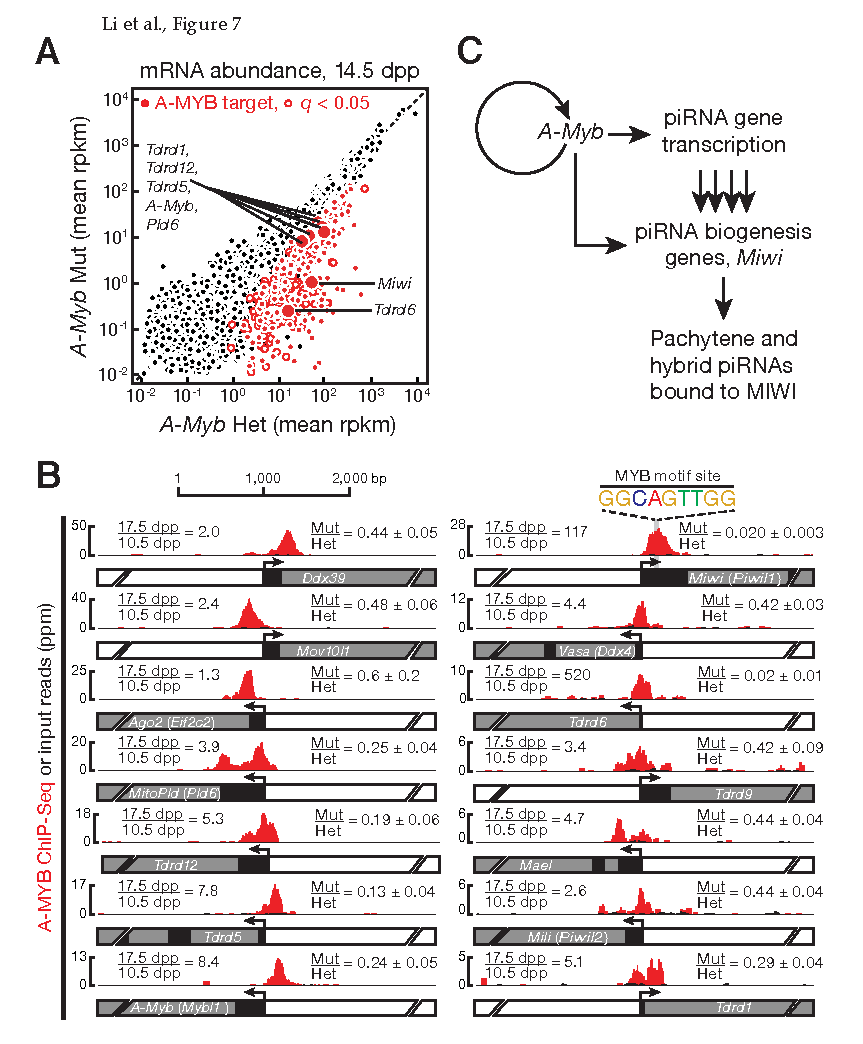
\includegraphics{Figures/MolCel/MolCel2013_Fig7.eps}
      \caption[A-MYB Regulates Expression of mRNAs Encoding piRNA Pathway Proteins]
      {
        See subsubsection \ref{MolCel:subsubsection:cap:Figure F7} for full figure caption.
      	}
      \label{MolCel:fig:MolCelF7}
    	\end{figure}

    \begin{figure} % Figure S7
      \centering 
      \includegraphics{Figures/MolCel/MolCel2013_FigS7.eps}
      \caption[\amyb{} mutants, but Not \miwi{} Mutants, Change the Expression of RNA Silencing Pathway Genes]
      {
      	See subsubsection \ref{MolCel:subsubsection:cap:Figure S7} for full figure caption.
      	}
      \label{MolCel:fig:MolCelS7}
    	\end{figure}

      \subsubsection{Caption for Figure \ref{MolCel:fig:MolCelF7}}
        \label{MolCel:subsubsection:cap:Figure F7}
        (A) mRNA abundance in \amyb{} mutant versus heterozygous testes. The 407 genes with a significant (q < 0.05) change in steady-state mRNA levels are shown as red circles. The 203 with A-MYB peaks within 500 bp of their transcription start site are filled.
        (B) A-MYB ChIP-seq signal at the transcription start sites of \amyb{} and genes implicated in RNA silencing pathways. For each, the figure reports the change in mRNA abundance between 17.5 and 10.5 dpp in wild-type testes and the mean change between \amyb{} mutant and heterozygous testes at 14.5 dpp (mean $\pm$ SD; n = 3).
        (C) A model for the regulation of pachytene piRNA biogenesis by A-MYB. See also Figure \ref{MolCel:fig:MolCelS7} and Table S3.

      \subsubsection{Caption for Figure \ref{MolCel:fig:MolCelS7}}
        \label{MolCel:subsubsection:cap:Figure S7}
        A) mRNA abundance in 17.5 dpp \amyb{} versus heterozygous testes. The 2,853 genes with a significant (q < 0.051) change in steady-state mRNA abundance are shown as open red circles. Among them, 8721,009 genes also had A-MYB peaks within 500 bp of their transcription start sites. These ``A-MYB targets'' are marked with filled red circles. (B) Same as (A) but in 14.5 dpp \miwi{} mutant versus heterozygous testes. The genes encoding proteins implicated in RNA silencing pathways that were labeled in (A) and that showed no change in expression in \miwi{} mutant testes are highlighted as green filled circles. As expected, \miwi{}, showed a significant decrease in mRNA abundance in \miwi{}-/- testes. (C) The change in mRNA abundance (rpkm) in \amyb{} and \miwi{} mutant testes versus heterozygous controls for the RNA silencing genes highlighted in (A) and (B).

  \subsection{Feed-Forward Regulation of piRNA Production is Evolutionarily Conserved}
    \label{MolCel:subsec:A-MYB in Chickens}

    Is A-MYB-mediated, feedforward control a general feature of regulation of piRNA production among vertebrates? To test whether A-MYB control of piRNA precursor transcription is evolutionarily conserved, we used high-throughput sequencing to identify piRNAs in adult rooster testes. Birds and mammals diverged 330 million years ago \citep{Benton2007}. After removing the sequences of identifiable miRNAs \citep{Burnside2008} and annotated noncoding RNAs, total small RNA from the adult rooster testis showed peaks at both 23 and 25 nt (Figure \ref{MolCel:fig:MolCelF8}A). When the RNA was oxidized before being prepared for sequencing, only a single 25 nt peak remained, consistent with the 25 nt small RNAs corresponding to piRNAs containing 2\textprime-O-methyl-modified 3\textprime~termini. These longer, oxidation-resistant species typically began with uracil (62\% of species and 65\% of reads; Figure \ref{MolCel:fig:MolCelF8}B), and we detected a significant Ping-Pong amplification signature (Z score = 31; Figure \ref{MolCel:fig:MolCelF8}C). We conclude that the oxidation-resistant, 24-30 nt long small RNAs correspond to rooster piRNAs. Like piRNAs generally, rooster piRNAs are diverse, with 5,742,529 species present among 81,121,893 genome-mapping reads. Like mouse pachytene piRNAs, 70\% of piRNAs from adult rooster testes mapped to unannotated intergenic regions, 19\% mapped to transposons, and 14\% mapped to protein-coding genes. Of the piRNAs that map to protein-coding genes, >95\% derive from introns. Forty-two percent of piRNA species mapped uniquely to the Gallus gallus genome.

    Using 24-30 nt piRNAs from oxidized libraries, we identified 327 rooster piRNA clusters (Figure \ref{MolCel:fig:MolCelS8}). These account for 76\% of all uniquely mapping piRNAs. Of the 327 clusters, 25 overlapped with protein-coding genes. To begin to identify the transcription start sites for the rooster piRNA clusters, we analyzed adult rooster testes by H3K4me3 ChIP-seq. More than 81\% (268 out of 327) of the clusters contained a readily detectable H3K4me3 peak within 1 kbp of the piRNA cluster. In contrast, the median distance from a cluster to the nearest transcription start site of an annotated gene was 73 kbp, suggesting that the H3K4me3 peaks reflect the start sites for rooster piRNA precursor transcripts.

    Next, we asked where in the genome A-MYB bound in adult rooster testes. A-MYB ChIP-seq identified 5,509 significant peaks (FDR < 10-25). MEME analysis of the top 500 peaks with the lowest FDR values identified a motif (E = 2.6 x 10-201; Figure \ref{MolCel:fig:MolCelF8}D) similar to that found in the mouse (Figure \ref{MolCel:fig:MolCelF4}A). A-MYB is the only one of the three chicken MYB genes expressed in adult testis (X.Z.L. and P.D.Z., unpublished data), supporting the view that these peaks correspond to A-MYB binding. The core sequence motif associated with A-MYB binding in mouse differs at one position (CAGTT) from that in rooster (C C/G GTT). This difference between mammalian and chicken MYB proteins has been noted previously \citep{Weston1992, Deng1996}.


    \begin{figure} % Figure 8
      \centering 
      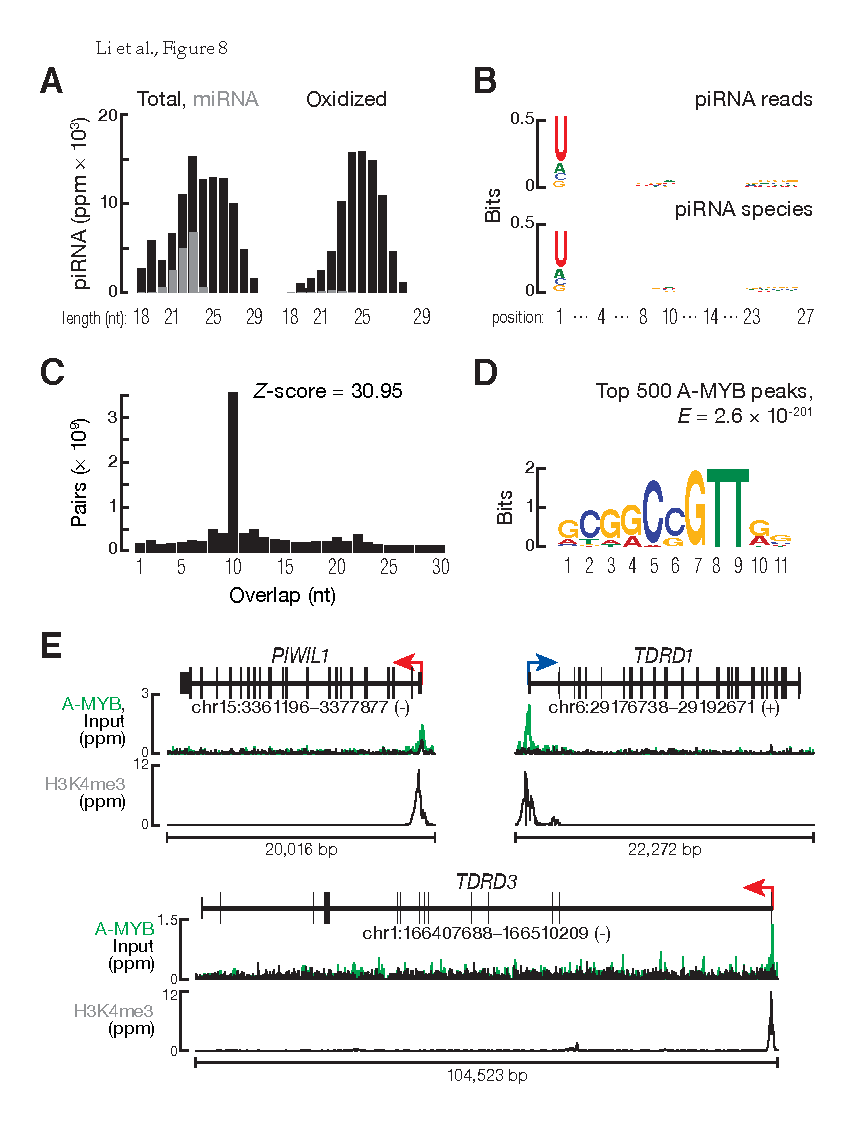
\includegraphics{Figures/MolCel/MolCel2013_Fig8.eps}
      \caption[Feed-Forward Regulation of piRNA Biogenesis by A-MYB is Conserved in Rooster]
      {
        See subsubsection \ref{MolCel:subsubsection:cap:Figure F8} for full figure caption.
      	}
      \label{MolCel:fig:MolCelF8}
    	\end{figure}
    \begin{figure} % Figure S8
      \centering 
      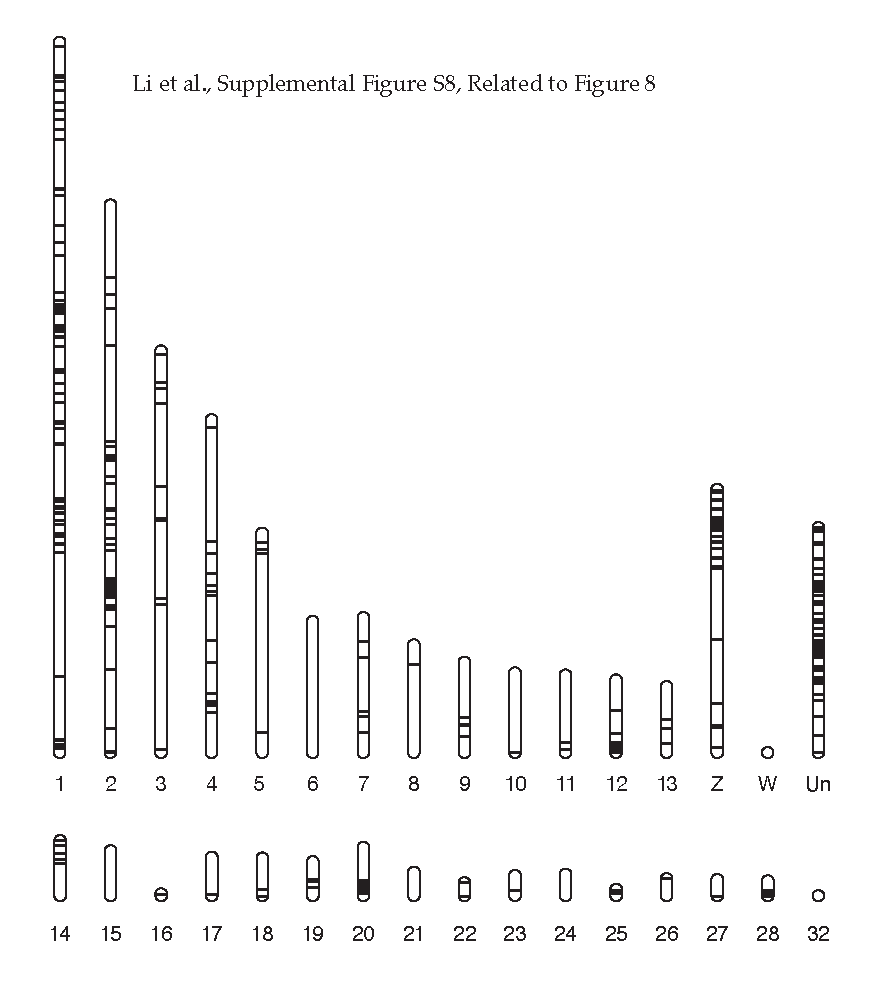
\includegraphics{Figures/MolCel/MolCel2013_FigS8.eps}
      \caption[Genomic Locations of piRNA Clusters in the Rooster (Gallus gallus) Testis.]
      {
     	 Black horizontal lines denote the locations on the Gallus gallus (galGal3) chromosomes of the piRNA clusters identified by small RNA sequencing. The figure shows 324 clusters; clusters on E64 (cluster 370) and E22C19W28_E50C23 (clusters 109 and 563) are not shown.
     	 }
      \label{MolCel:fig:MolCelS8}
    	\end{figure}

    To determine whether chicken A-MYB might regulate transcription of some piRNA clusters in the testis, we compared the A-MYB peak nearest to each piRNA cluster with the nearest H3K4me3 peak. Of the 327 rooster piRNA clusters, at least 104 were occupied by A-MYB at their promoters, as defined by an overlapping H3K4me3 peak. These 104 clusters account for 31\% of uniquely mapping rooster piRNAs.

    The chicken genome encodes at least two PIWI proteins: PIWIL1 and PIWIL2. Remarkably, the promoter of Gallus gallus PIWIL1, the homolog of mouse \miwi{}, contained a prominent A-MYB peak (Figure \ref{MolCel:fig:MolCelF8}E). TDRD1 and TDRD3 also showed A-MYB peaks (Figure \ref{MolCel:fig:MolCelF8}E). Thus, as in mice, Gallus gallus A-MYB controls the transcription of both piRNA clusters and genes encoding piRNA pathway proteins. We conclude that A-MYB-mediated feedforward regulation of piRNA production was likely present in the last common ancestor of birds and mammals.

    In mice, we found no piRNA-producing genes on the sex chromosomes (Figure \ref{MolCel:fig:MolCelS1}A), perhaps because mouse sex chromosomes are silenced during the pachytene stage \citep{Li2009d}. Birds use a ZW rather than an XY mechanism for sex determination, so roosters are homogametic (ZZ), allowing the sex chromosomes to remain transcriptionally active in males \citep{Namekawa2009, Schoenmakers2009}. Indeed, we find that 39 of the 327 rooster piRNA clusters are on the Z chromosome, accounting for 12\% of uniquely mapping piRNAs (Figure \ref{MolCel:fig:MolCelS8}). Of the 39 Z chromosome clusters, 18 had an A-MYB peak at their promoter.

    \subsubsection{Caption for figure \ref{MolCel:fig:MolCelF8}}
    \label{MolCel:subsubsection:cap:Figure F8}
      (A) Length distributions of total rooster testis small RNAs (black) and miRNAs (gray).(B) Sequence logo showing the nucleotide composition of piRNA reads and species.(C) The 5\textprime~-5\textprime~overlap between piRNAs from opposite strands was analyzed to determine if rooster piRNAs display Ping-Pong amplification. The number of pairs of piRNA reads at each position is reported. Z score indicates that a significant 10 nt overlap (Ping-Pong) was detected. Z score > 1.96 corresponds to p value < 0.05.(D) MEME-reported motif of the top 500 (by peak score) A-MYB ChIP-seq peaks from adult rooster testes.(E) A-MYB, H3K4me3, and input ChIP-seq signals at the transcription start sites of rooster PIWIL1, TDRD1, and TDRD3. See also Figure S8.

\section{Discussion}
  \label{MolCel:sec:Discussion}

  The data presented here provide strong support for the view that piRNAs in mammals begin as long, single-stranded precursors generated by testis-specific, RNA Pol II transcription of individual piRNA genes (see also \citet{Vourekas2012}. Transcription by RNA Pol II affords piRNA genes the same rich set of transcriptional controls available to regulate mRNA expression. Our data establish that developmentally regulated transcription of piRNA genes determines when specific classes of piRNAs emerge during spermatogenesis.

  During mouse spermatogenesis, transcription of pachytene piRNA genes begins at the onset of the pachytene stage of meiosis; pachytene piRNAs accumulate subsequently. The presence of the MYB binding motif near the transcription start sites of pachytene piRNA genes, the physical binding of A-MYB to those genes, and the loss of pachytene piRNA precursor transcripts and piRNAs in testes from \amyb{} mutant mice all argue that A-MYB regulates pachytene piRNA production.

  A-MYB also drives increased expression of piRNA pathway genes. Among these, \miwi{} expression shows the greatest dependence on A-MYB, but A-MYB also drives transcription of genes encoding other proteins in the piRNA pathway, including MitoPld, Mael, and five genes encoding Tudor domain proteins. For example, A-MYB increases expression of Tdrd6 more than 500-fold. Loss of A-MYB function more strongly depletes pachytene piRNAs than loss of MIWI, in part because pachytene piRNAs can still be loaded into MILI in \miwi{} mutant testes, although MILI-loaded pachytene piRNAs do not suffice to produce functional sperm. In the \amyb{} mutant, expression of mRNAs encoding multiple piRNA pathway proteins decreases. We speculate that in wild-type male mice, the increased expression of these mRNAs at the onset of the pachytene stage of meiosis ensures that sufficient piRNA-precursor-processing and MIWI-loading factors are available to cope with the large increase in pachytene piRNA precursor transcription.

  We propose that induction of A-MYB during the early pachytene stage of spermatogenesis initiates a feedforward loop that ensures the precisely timed production of these piRNAs. Coherent feedforward loops show delayed kinetics in order to reject background stimuli \citep{Mangan2003}. Indeed, we observed a delay from the early to middle pachytene in the accumulation of pachytene piRNAs, despite the continued increase in \amyb{} expression (Figure \ref{MolCel:fig:MolCelF2}A). Pachytene piRNA levels increase 75-fold (median for the 100 genes) from 10.5 to 12.5 dpp, coincident with increased expression of \amyb{}. However, from 12.5 to 14.5 dpp, pachytene piRNAs increase only 1.2-fold. Pachytene piRNAs subsequently resume their accumulation, increasing 65-fold from 14.5 to 17.5 dpp. We believe this delay is a consequence of a feedforward loop that ensures the production of pachytene piRNAs only at the pachytene stage of spermatogenesis. Regulation by a feedforward loop also predicts a rapid shutdown of pachytene piRNA pathways at round spermatid stage VIII, when A-MYB protein levels decrease \citep{Horvath2009}. Supporting this idea, the abundance of MIWI decreases sharply by the elongated spermatid stage of spermatogenesis \citep{Deng2002c}. Testing this proposal is a clear challenge for the future.

  In fruit flies and zebrafish \citep{Brennecke2007, Houwing2007}, most piRNAs map to repetitive regions, whereas in mammals, uniquely mapping intergenic piRNAs predominate in the adult testis. The discovery that 70\% of rooster piRNA reads map to intergenic regions suggests that the expansion of intergenic piRNAs controlled by A-MYB feedforward regulation arose before the divergence of birds and mammals. In the future, detailed analysis of piRNA production across avian spermatogenesis should provide insight into the evolutionary origins and functions of pachytene piRNAs, a class of piRNAs thus far only detected in mammals.

  In summary, we have shown that mouse piRNA genes are coregulated transcriptionally, establishing that A-MYB coordinately regulates the biogenesis of an entire piRNA class, the pachytene piRNAs. The discovery that a loss-of-function \amyb{} mutant, \mybrepro{}, disrupts piRNA precursor transcription in vertebrates provides a tool to understand the transformation of long, single-stranded piRNA precursors into mature piRNAs and to explore the functions and targets of the pachytene piRNAs.

\section{Experimental Procedures}
  \label{MolCel:sec:Experimental Procedures}

  \begin{description}
    \item[Mice] \hfill \\
    \mybrepro{}, \textit{\spo{}}$^{tm1Sky}$, and \textit{Piwil1}$^{tm1Hf}$ mice were maintained and used according to the guidelines of the Institutional Animal Care and Use Committee of the University of Massachusetts Medical School and genotyped as described \citep{Baudat2000c, Deng2002c, Bolcun-Filas2011}.

    \item[Sequencing] \hfill \\
    Small \citep{Ghildiyal2008, Seitz2008} and long RNA-seq \citep{Zhang2012a} and analysis \citep{Li2009a} were as described. Reads that did not map to mouse genome mm9 were mapped to piRNA precursor transcripts to obtain splice junction mapping small RNAs. Total small RNA libraries from different developmental stages and from mutants were normalized to the sum of all miRNA hairpin mapping reads. Oxidized samples were calibrated to the corresponding total small RNA library via the abundance of shared, uniquely mapped piRNA species. piRNA expression data were grouped with Cluster 3.0. Differential gene expression was analyzed with DESeq R \citep{Anders2010a}; ChIP-seq reads were aligned to the genome using Bowtie version 0.12.7 \citep{Langmead2009}, and peaks were identified using MACS \citep{Zhang2008}.

    \item[Acknowledgments] \hfill \\
    We thank K. Chase and K. Schimenti for help collecting tissues; C. Tipping for help with mouse husbandry; P. Johnson and B. Keagle for providing rooster testes; G. Farley for technical assistance; H. Lin for reagents; Xi Chen, Xiaotu Ma, Oliver Rando, and Benjamin Carone for advice on ChIP; and members of our laboratories for critical comments on the manuscript. X.Z.L. was supported by the Lalor Foundation and the Jane Coffin Childs Memorial Fund for Medical Research.

    \item[Accession Numbers] \hfill \\
    The Gene Expression Omnibus (GEO) accession number for the RNA-seq, ChIP-seq, and small RNA data reported in this paper is GSE44690.

    \item[Animals] \hfill \\
    Mice were maintained and used according to the guidelines of the Institutional Animal Care and Use Committee of the University of Massachusetts Medical School. C57BL/6J (Jackson Labs, Bar Harbor, ME, USA; stock number 664); \mybrepro{} in a mixed 129X1/SvJ x C57BL/6J background; Spo11tm1Sky in a C57BL/6J background; and Piwil$^{1tm1Hf}$ in a mixed 129X1/SvJ x C57BL/6J background (``\miwi{}'') mice were genotyped as described \citep{Baudat2000c, Deng2002c, Bolcun-Filas2011}. Rooster testes from White Leghorn of the Cornell Special C strain, about 15 months old, were used for small RNA analysis; and testes from the Brown Leghorn strain, about one year old, were used for ChIP analysis.

    \item[RNA Sequencing] \hfill \\
    Small RNA libraries were constructed and sequenced as described \citep{Ghildiyal2008, Seitz2008} except that 18-35 nt RNA was isolated and 2S rRNA depletion omitted. Sequencing was performed using either a Genome Analyzer GAII (36 or 76 nt reads) or HiSeq 2000 (50 nt) instrument (Illumina, San Diego, CA, USA). We analyzed published small RNA libraries from purified mouse spermatogonia (SRR069809), spermatocytes (SRR069810, GSE39652), or spermatids (SRR069811; \citep{Gan2011, Modzelewski2012}; from \mili{} mutant or heterozygous testes at 10 dpp (SRX003089 and SRX003088; \citep{Aravin2008a}; from Tdrd6 mutant or heterozygous testes at 18 dpp (SRX012165 and SRX012166; \citep{Vagin2009}; and MILI IP samples from Tdrd9 mutant or heterozygous testes at 14 dpp (SRX015795, SRX015796, SRX015797, and SRX015798; \citep{Shoji2009}.

    Strand-specific RNA-seq libraries \citep{Zhang2012} using Ribo-Zero Gold (Epicentre Biotechnologies, Madison, WI, USA) were sequenced using the paired-end protocol on a HiSeq 2000.
    
    \item[Small RNA Analysis] \hfill \\
    Small RNA sequence analysis was as described \citep{Li2009a} using mouse genome release mm9 and chicken genome release galGal3. Non-coding RNA annotations comprised data from ncRNAscan, the known tRNAs from UCSC, and 18S, 28S and 5.8S rRNAs. miRNA hairpin and mature miRNA annotation was from miRBase Release 19. Mouse and chicken transposons were annotated using Repeat Masker from UCSC. Reads that did not map to the mouse genome (mm9) were mapped to piRNA precursor transcripts to obtain splice junction-mapping small RNAs. Total small RNA libraries from different developmental stages and from mutants were normalized to the sum of all miRNA hairpin-mapping reads. Oxidized samples were calibrated to the corresponding total small RNA library via the abundance of shared, uniquely mapped piRNA species. Table S1 reports the statistics for high-throughput sequencing. For oxidized (i.e., piRNA-enriched) samples, uniquely mapping small RNAs >23 nt were mapped to each assembled piRNA precursor transcript and reported as reads per kilobase pair per million reads mapped to the genome (rpkm) using a pseudo count of 0.001.

    \item[Small RNA Analysis] \hfill \\
    RNA-seq reads were aligned to the genome (NCBI 37/mm9) using TopHat 2.0.4 \citep{Trapnell2009}. Reads were mapped uniquely using the ``-g 1'' switch. We assembled the mouse testes transcriptome (see below). For genes with multiple isoforms, the transcript with the highest average rpkm value among the three replicates of adult testes was selected for further analysis. Fragments with both reads mapped within a transcript, or to piRNA precursor transcripts, were counted using BEDTools \citep{Quinlan2010}. The sum of the reads aligning to the top quartile of expressed transcripts per library was used to calibrate the samples. The number of reads per transcript was normalized by length, divided by the library-specific calibration factor, and reported as rpkm with a pseudo count of 0.001. Table S1 presents the statistics for the RNA-seq data. Sequences mapping to five genes (Table S1) that overlapped with or were embedded within a piRNA gene were excluded when calculating piRNA precursor transcript abundance.

    \item[PAS-seq Library Construction and Analysis] \hfill \\
    PAS-seq libraries (Table S1) were prepared essentially as described \citep{Shepard2011} and sequenced using a HiSeq 2000 (100 nt read length). We first removed adaptors and performed quality control using Flexbar 2.2 (http://sourceforge.net/projects/theflexibleadap) with the parameters ``-at 3 -ao 10 --min-readlength 30 --max-uncalled 70 --phred-pre-trim 10.'' For reads beginning with GGG including (NGG, NNG or GNG) and ending with three or more adenosines, we removed the first three nucleotides and mapped the remaining sequence with and without the tailing adenosines to the mouse genome using TopHat 2.0.4. We retained only those reads that could be mapped to the genome without the trailing adenosine residues. Genome-mapping reads containing trailing adenosines were regarded as potentially originating from internal priming and thus discarded. The 3\textprime~end of the mapped, retained read was reported as the site of cleavage and polyadenylation.

    \item[CAGE Library Construction and Analysis] \hfill \\
    CAGE (cap analysis of gene expression; Table S1) was as described \citep{Yang2011} and sequenced using a HiSeq 2000 (100 nt reads). After removing adaptor sequences and checking read quality using Flexbar 2.2 with the parameters of 
    \lstset{language=BASH}
    \begin{lstlisting}
    -at 3 -ao 10 --min-readlength 20 --max-uncalled 70 --phred-pre-trim 10
    \end{lstlisting}
    , we retained only reads beginning with NG or GG (the last two nucleotides on the 5\textprime~adaptor). We then removed the first two nucleotides and mapped the sequences to the mouse genome using TopHat 2.0.4. All unique 5\textprime~ends of the mapped positions were considered as CAGE-tag starting sites and grouped into tag clusters using a distance-based method in which the maximal distance between two neighboring tags was required to be <20 bp. The peak position of a tag cluster was then reported as the transcription start site.

    \item[Transcriptome Assembly and Annotation] \hfill \\
    De novo transcriptome assembly from three biological replicates of strand-specific RNA-seq data from adult testes was performed using Trinity (r2012-06-08) with default parameters \citep{Grabherr2011}. The assembled RNA sequences were aligned to the mouse genome (mm9) with BLAT \citep{Kent2002}, and the alignments with more than 95\% of sequence length mapped and fewer than 1\% mismatches retained.

    We extracted novel junctions from Trinity (i.e., reads with [0-9]+M[0-9]+N[0-9]+M pattern in the CIGAR string of SAM output), and re-mapped all RNA-seq reads to these junctions, rescuing 1,402,444 reads in three replicates. Rescued reads were combined with TopHat alignments (supplied with ``-max-multihits 100'' to assembly through repetitive regions) and used as input for reference-based assembly.

    We used Cufflinks v2.0.2 \citep{Trapnell2010} with parameters of:
    \lstset{language=BASH}
    \begin{lstlisting}
    -u -j 0.2 --min-frags-per-transfrag 40
    \end{lstlisting}
    to assemble transcripts. To join small transcript fragments caused by insufficient read coverage or embedded repetitive elements, two different gap-joining distance cutoffs were used for the assembly of genes (``\-\-overlap-radius 100'') and piRNA loci (``--overlap-radius 250''). We used Cuffcompare v2.0.2 \citep{Trapnell2010} to annotate the 49,840 Cufflinks-assembled transcripts using parameters optimized for genic conditions (``\-\-overlap-radius 100'').

    \item[piRNA Precursor Transcript Annotation] \hfill \\
    We combined transcripts from the two Cufflink assemblies with those from the Trinity assembly, producing 136,069 unique transcripts. Those transcripts with 100 ppm or 100 rpkm unique mapping piRNAs at any time point (10.5, 12.5, 14.5, 17.5, 20.5 dpp and adult oxidized small RNA from testis) were selected for manual annotation.

    To refine the termini of the piRNA-producing transcripts, we supplemented the RNA-seq data with high-throughput sequencing of 5\textprime~ends of RNAs bearing (5\textprime~)ppp(5\textprime~) cap structures (CAGE) and of the 3\textprime~ends of transcripts flanking the poly(A) tail (PAS-seq). To provide independent confirmation of the 5\textprime~ends of each piRNA-producing transcript, we used chromatin immunoprecipitation (ChIP-seq) of RNA polymerase II (pol II) and histone H3 bearing trimethylated lysine-4 (H3K4me3). Refinement of transcriptional starts required both a CAGE and a H3K4me3 peak to support the 5\textprime~end of the transcript. When no H3K4me3 peak corroborated alternative transcription start sites proposed by the CAGE data, the alternative transcripts were merged with the fully substantiated transcript.

    \item[piRNA Gene Nomenclature] \hfill \\
    When piRNA-producing genes overlap an annotated protein coding gene, we refer to them using the name of the overlapping gene preceded by ``pi-''; when they do not, their names refer to their genomic location followed by a number indicating the piRNA abundance in ppm at 6 weeks post-partum. The last digit of a piRNA gene name specifies the rank order of expression among isoforms, determined by the highest abundance of transcripts (rpkm) observed for that gene among the six developmental stages of testis.

    \item[Grouping piRNA Precursor Transcripts] \hfill \\
    For the most abundant transcript in each locus, the abundance (rpkm) of piRNAs at each stage was expressed as a fraction of the maximum abundance reached during the developmental time course. These data were then analyzed by hierarchical clustering according to Euclidean distance and complete linkage using Cluster 3.0. Clustering results were visualized using Java Tree View 1.1.3.

    \item[Analysis of Differential Gene Expression ] \hfill \\
    We determined differential gene expression using DESeq R \citep{Anders2010a}. For each annotated mRNA, reads from each library were aligned to the most abundant assembled transcript. Transcripts with q < 0.05 were considered to be differentially expressed. Table S3 lists the genes that were differentially expressed in \amyb{} at 14.5 dpp. Three biologically independent replicates were used for \amyb homozygotes and heterozygotes at 14.5 and at 17.5 dpp.

    \item[Motif Discovery] \hfill \\
    For divergently transcribed piRNA gene pairs, the promoter region was defined as the region between the transcription start sites defined by CAGE peaks. Sequence motifs in these putative promoter regions were detected ab initio using MEME \citep{Bailey1994, Bailey2009} in TCM mod (any number of repetitions per sequence) and compared to existing JASPAR and TRANSFAC libraries via TOMTOM \citep{Gupta2007}. FIMO was used to detect motif sites within the putative promoters (default p < 10$^{-4}$; \citep{Grant2011}.

    \item[Chromatin Immunoprecipitation (ChIP)] \hfill \\
    ChIP was performed as described \citep{Chen2008} except that testes were macerated on ice and then fixed with 1.5\% (w/v) formaldehyde for 20 min. Samples were then further crushed using 20 strokes with a ``B'' pestle in a Dounce homogenizer (Kimble-Chase, Vineland, NJ, USA). Chromatin was sheared by sonication and immunoprecipitated using anti-A-MYB (HPA008791; Sigma, St. Louis, MO, USA) or anti-H3K4me3 (ab8580; Abcam, Cambridge, MA, USA) antibody; immunoglobulin G (IgG; Sigma, item 2729) served as a control. ChIP-quantitative PCR (qPCR) was performed using the CFX96 Real-Time PCR Detection System with SsoFast EvaGreen Supermix (Bio-Rad, Hercules, CA, USA). Data were analyzed using DART-PCR \citep{Peirson2003}. Relative ChIP enrichment values were normalized to \textit{MyoD1}, a gene not expressed in testes. Table S1 lists ChIP-qPCR primers. ChIP-seq libraries for anti-A-MYB and control input DNA were prepared following the Illumina ChIP-seq protocol and sequenced on a HiSeq 2000 (50 nt reads).

    \item[ChIP-seq Analysis] \hfill \\
    ChIP-seq reads were aligned to the genome using Bowtie version 0.12.7 \citep{Langmead2009}. Reads were mapped uniquely using the ``-M 1 --best --strata'' switches and one mismatch was allowed (-v 1). ChIP peaks were identified using MACS version 1.4.1 \citep{Zhang2008} using default arguments, input as control, and a cutoff p-value = 10$^{-25}$ was used. BEDTools was used to assign peaks to the nearest 5\textprime~end of genes. Table S1 reports sequencing statistics for ChIP-seq.

    \item[RT-PCR] \hfill \\
    Total RNA was treated with Turbo DNase (Ambion, Austin, TX, USA), and then reverse transcribed using SuperScript III (Invitrogen, Eugene, OR, USA) with random primers (Promega, Madison, WI, USA). The resulting cDNA was analyzed by conventional PCR. Table S1 lists the primers used in Figure \ref{MolCel:fig:MolCelS6}.

    \item[Ping-Pong Analysis] \hfill \\
    Ping-Pong amplification was analyzed by the 5\textprime~-5\textprime~overlap between piRNA pairs from opposite genomic strands \citep{Li2009a}. Overlap scores for each overlapping pair were the product of the number of reads of each of the piRNAs from opposite strands. The overall score for each overlap extend (1-30) was the sum of all such products for all chromosomes. Heterogeneity at the 3\textprime~ends of small RNAs was neglected. Z-score for 10 bp overlap was calculated using the scores of overlaps from 1-9 and 11-30 as background.

    \item[Rooster piRNA Cluster Detection] \hfill \\
    We developed a dynamic programming algorithm to identify the genomic regions with the highest piRNA density. We used oxidized small RNA reads (>23 nt) to detect clusters. We used the conservative assumption that piRNA clusters compose at most 2\% of the chicken genome. We first split the genome into 1 kbp non-overlapping windows and computed piRNA abundance for each window. The mean of the top 2\% of windows was used as the penalty score for the dynamic programming algorithm. The algorithm computes the cumulative piRNA abundance score as a function of the window index along each chromosome. The score at a window is the sum of the score in the previous window and the piRNA abundance in the current window, minus the penalty score; if the resulting score was negative it was reset to 0. The maximal score points to the largest piRNA cluster. We extracted the largest piRNA cluster, recomputed the scores at the corresponding windows, and searched for the next cluster. The process continued until the scores for all windows were zero. The boundaries of each cluster were further refined by including those base pairs for which piRNA abundance exceeded the mean piRNA abundance of the top 2\% windows. We considered only those clusters with abundance >10 ppm for uniquely mapping piRNAs. In Figure \ref{MolCel:fig:MolCelF8}E, gene models were corrected using data from our unpublished adult rooster testis RNA-seq data.

  	\end{description}

\cleardoublepage